\documentclass[12pt]{report}
\usepackage{setspace}  %use this package to set linespacing as desired
\usepackage{array}
\usepackage{graphicx}
\usepackage{subcaption}
\usepackage{amsmath}
\usepackage{color,soul}
\soulregister\cite7
\soulregister\ref7
\soulregister\pageref7
\usepackage[counterclockwise, figuresleft]{rotating}

\begin{document}
\doublespacing

\clearpage
\chapter{Methodology} \label{chapter:methodology}

\textbf{Things Still Needed:}
\begin{itemize}
\item Intro needed for Section \ref{section:datacollection}
\end{itemize}

\hl{This chapter contains the research methodology employed while implementing a proof-of-concept of an adaptive shadow removal model. Our methodology is divided into two components: algorithm assessment in the context of shadow removal in diverse environments, and the creation of the adaptive model for a previously assessed algorithm. 

We first assess the previously catalogued algorithms (Chromacity, Physical, Geometry, SRT, and LRT removal) for sensitivity to both environmental and parametric change. We then perform a similar sensitivity analysis upon the parameters utilized by the algorithms. These assessments are performed qualitatively to determine the feasibility of an adaptive model being created for each algorithm.} 

\hl{From the sensitivity assessments, we demonstrate the creation of an adaptive model for a previously analyzed algorithm parameter. The process of creating an  adaptive model, outlined in section \ref{section:adaptivemodelapproach}, is then detailed. We consider various environmental properties and evaluate their correlations to the selected algorithm parameter. Potential indirect correlative factors are detailed in sections \ref{section:brightnessmodels} and \ref{section:lowcSIFT}. Finally, methodology concerning assembling the adaptive model follows in section \ref{section:model}.}

\section{Algorithm Assessment}

\hl{We assess several leading shadow removal algorithms (Chromacity, Physical, Geometry, SRT, and LRT removal) for their sensitivity to different environmental properties, as well as quantitative shifts in those environmental properties. Environmental properties are identified across diverse datasets, examples including shadow strength/darkness, shadow directionality, and color saturation. Environmental property shifts are characterized in multiple datasets, i.e., strong illumination changes within one dataset sequence.

In addition to analyzing the algorithms' sensitivity to environmental change, we similarly assess the algorithms' sensitivity to parametric shift, i.e., algorithm performance is qualitatively assessed according to the algorithm's dependence on one or more curated parameter values. Analysis and assessment of the previously presented shadow removal algorithms is conducted using a series of graphical tools in conjunction with ground truths identifying shadow regions across eight different datasets with seven unique environments.}

\subsection{Data Collection and Analysis}  \label{section:datacollection}

What kind of introduction does the data collection section need?

\subsubsection{Datasets}
\hl{A total of eight datasets were chosen for this assessment, and are summarized in Table \ref{table:datasets}.} Datasets 2 - 8 (denoted by the prefix "aton\_") are provided under the Computer Vision and Robotics Research Laboratory (CVRR) in association with the University of San Diego [\ref{CVRR}]. The datasets were cataloged with the Autonomous Agents for On-Scene Networked Incident Management (ATON) project [\ref{aton}]. \hl{These datasets represent diverse environments, including both indoor and outdoor scenes, a range of shadow intensity, and images of varying saturation.}

\hl{In addition, two datasets were included from the Performance Evaluation of Tracking and Surveillance (PETS) project [\ref{pets}]. In contrast to the ATON datasets, these sequences were explicitly chosen because they possess subsequences featuring rapid illumination changes, due to a shift in weather conditions and cloud cover. These environmental changes darken, lighten, and blend shadows in accordance with a background model. Figure \ref{fig:pets2illum} demonstrates the illumination changes within the PETS datasets.}

\hl{All eight datasets} were manually segmented to form ground truths that identify shadow regions (gray) within foreground objects (white). \hl{Figure \ref{fig:datasetsgt} illustrates the ground truths of dataset frames.}

\hl{The .avi sequences aren't hosted where they were, meaning I probably can not find the sequence length.}

\begin{table}
\centering
\begin{tabular}{ |c|c|c| }
	\hline
	\textbf{Name} & \textbf{Resolution} & \textbf{\# Ground Truth Frames} \\
	\hline
	\hline
	PETS1 & 768x576 & 12 \\
	\hline
	PETS2 & 768x576 & 11 \\
	\hline
	aton\_highway1 & 320x240 & 8 \\
	\hline 
	aton\_highway3 & 320x240 & 7 \\ 
	\hline
	aton\_room & 320x240 & 22 \\ 
	\hline
	aton\_campus & 320x240 & 53 \\ 
	\hline
	aton\_hallway & 320x240 & 13 \\
	\hline
	aton\_lab & 320x240 & 14 \\ 
	\hline
\end{tabular} \label{table:datasets}
\caption{Dataset information.}
\end{table}

\begin{figure}
\centering
\begin{subfigure}{.3\linewidth}
  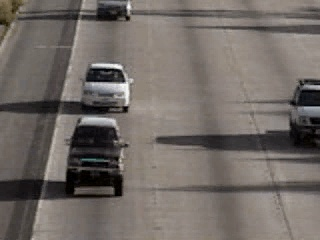
\includegraphics[width=1\linewidth]{figures/highway1_0045.jpg}
\end{subfigure}
\hfill
\begin{subfigure}{.3\linewidth}
  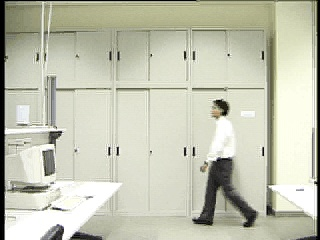
\includegraphics[width=1\linewidth]{figures/lab_0151.jpg}
\end{subfigure}
\hfill
\begin{subfigure}{.3\linewidth}
  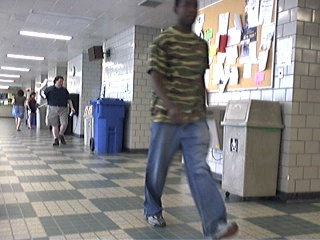
\includegraphics[width=1\linewidth]{figures/hallway_0164.jpg}
\end{subfigure}
\hfill
\begin{subfigure}{.3\linewidth}
  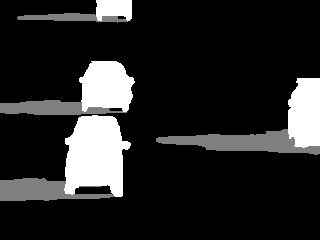
\includegraphics[width=1\linewidth]{figures/highway1_gt_0045.jpg}
  \caption{}
\end{subfigure}
\hfill
\begin{subfigure}{.3\linewidth}
  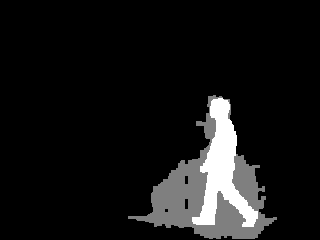
\includegraphics[width=1\linewidth]{figures/lab_gt_0151.jpg}
  \caption{}
\end{subfigure}
\hfill
\begin{subfigure}{.3\linewidth}
  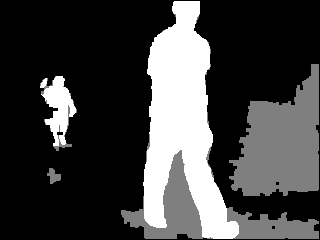
\includegraphics[width=1\linewidth]{figures/hallway_gt_0164.jpg}
  \caption{}
\end{subfigure}

\caption{Datasets collected for ATON: (a) aton\_highway1, (b) aton\_lab, and (c) aton\_hallway.}
\label{fig:datasetsgt}
\end{figure}

\begin{figure}
\centering
\begin{subfigure}{.48\linewidth}
  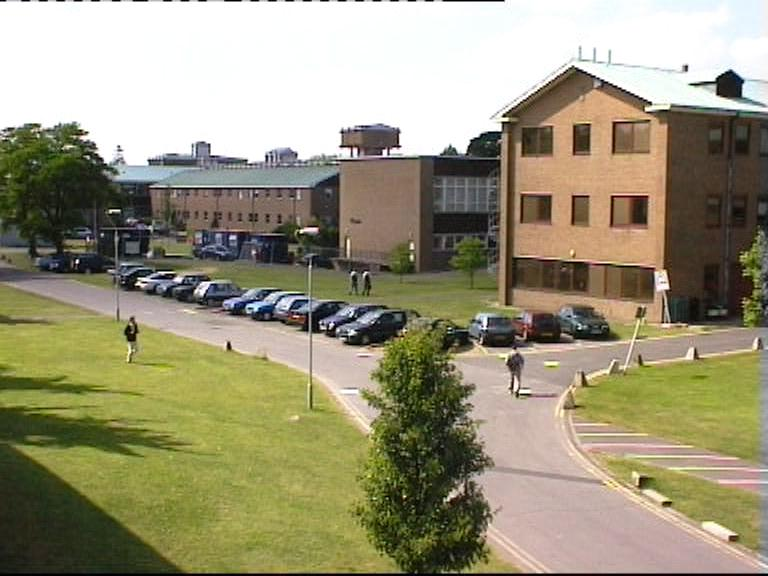
\includegraphics[width=1\linewidth]{figures/PETS2_highv.jpg}
  \caption{}
  \label{fig:sub1}
\end{subfigure}
\hfill
\begin{subfigure}{.48\linewidth}
  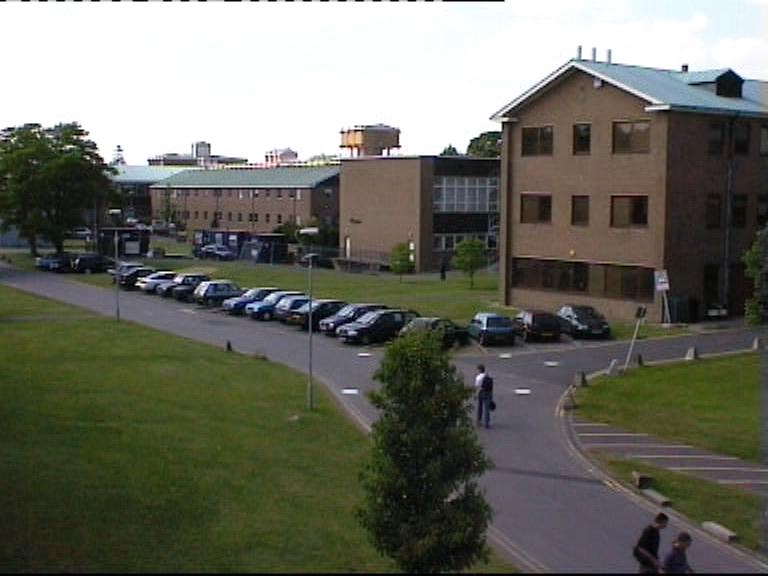
\includegraphics[width=1\linewidth]{figures/PETS2_lowv.jpg}
  \caption{}
  \label{fig:sub2}
\end{subfigure}
\caption{PETS2 experiencing both high illumination (a) and low illumination (b) (due to cloud cover).}
\label{fig:pets2illum}
\end{figure}

\subsubsection{Assessment Tools}

\hl{The first stage of our methodology is an exploration of the sensitivity of shadow removal algorithms to environmental and parametric change. We developed tools to assist intuition regarding an algorithm's performance, capable of allowing a user to manually tune an algorithm parameter, and observe its effect on performance.}

\hl{To better understand an algorithm's dependence on a parameter, a framework was required to rapidly modify the parameter in question. The initial implementation of the shadow removal methods, courtesy of Sanin et al. [\ref{alg impl}], contained relevant parameters hard-coded into the algorithms.} Each algorithm therefore required re-compilation to bring any modifications to fruition. This shortcoming was rectified by extracting each parameter and organizing them into an \textit{.ini} file. By utilizing \hl{username} \textit{brofield}'s SimpleINI architecture, hosted on Github [\ref{brofield}], parameters can be either set extemporaneously or altered by an external script. An example SimpleIni .ini file is shown in Figure \ref{fig:simpleini}.

\begin{figure}
  \centering
  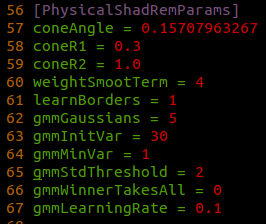
\includegraphics[width=.5\linewidth]{figures/simpleini.png}
  \caption{An example SimpleINI file. Parameters taken from this file are used to adjust values in real-time.}
  \label{fig:simpleini}
\end{figure}

\hl{Graphical tools (GUI) were then developed to rapidly assess and visualize a parameter's affect on shadow removal. Each shadow removal method was modified to accept arbitrary parameter values in real-time from the .ini file. These parameters were then tied to graphical sliders (from OpenCV's highgui library [\ref{opencvhighgui}]) dictating their range and value. Any numerical parameter that has the potential to modify the Detection or Discrimination rates of a shadow removal method is included in the GUI. An example of the GUI is seen in Figure \ref{fig:guitools}. The process in which the GUI modifies and displays parameters is illustrated in Figure \ref{fig:guimodel}.}

\begin{figure}
\centering
\begin{subfigure}{.49\linewidth}
  \centering
  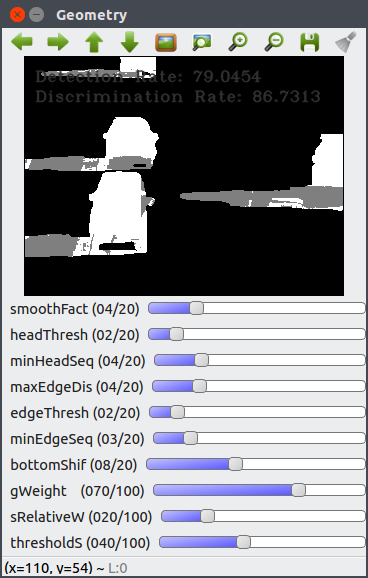
\includegraphics[width=.7\linewidth]{figures/geo_highway1_default.png}
\end{subfigure}
\hfill
\begin{subfigure}{.49\linewidth}
  \centering
  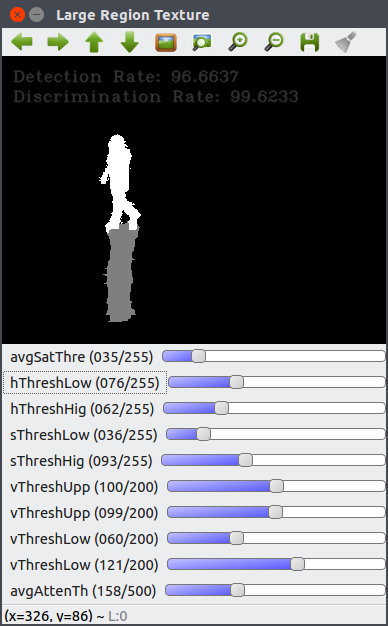
\includegraphics[width=.7\linewidth]{figures/lr_caviar_default.png}
\end{subfigure}
\caption{GUI tools created using OpenCV, displaying Geometry removal and LRT removal.}
\label{fig:guitools}
\end{figure}

\begin{figure}
  \centering
  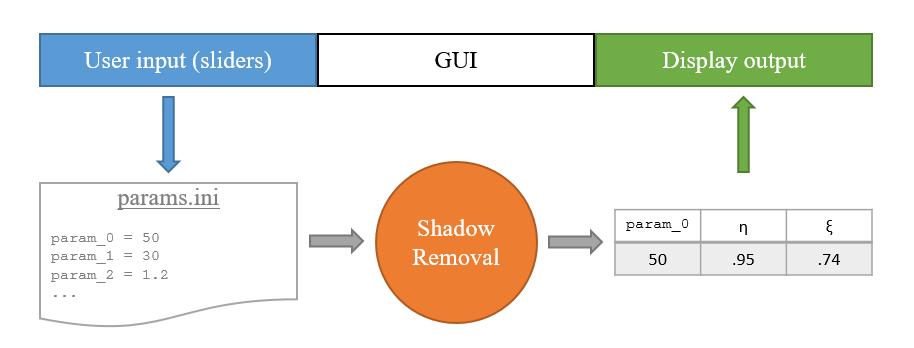
\includegraphics[width=1\linewidth]{figures/gui_model.png}
  \caption{The GUI takes user input through sliders, updates values in a .ini file, which are used to produce new detection and discrimination rates. The GUI then visualizes this output.}
  \label{fig:guimodel}
\end{figure}

The display is updated in real-time with both a visual representation of detected shadow pixels, and a quantified display of both the exact detection and discrimination rates. \hl{Leveraging human perception} \hl{(qualitative perception?)}, the graphical tools enabled rapid evaluation of the sensitivity of an algorithm to changes in parameter values within specific scenes.

%%%
\subsubsection{Determining Optimal Parameter Values}
%%%

\hl{The removal of compilation enables us to create batch jobs to systematically vary parameter values across multiple runs. This allows us to meticulously exercise a given parameter ($pr$) through a specified range and record its corresponding affect upon detection and discrimination rates. Figure \ref{fig:guiiterate} illustrates the data collection process. The calculated detection and discrimination responses to change in $pr$ are recorded as the functions $\eta(pr)$ and $\xi(pr)$. Both $\eta(pr)$ and $\xi(pr)$ are determined for one frame. Figure \ref{fig:campusddscore}(a) demonstrates these responses.}

\begin{figure}
  \centering
  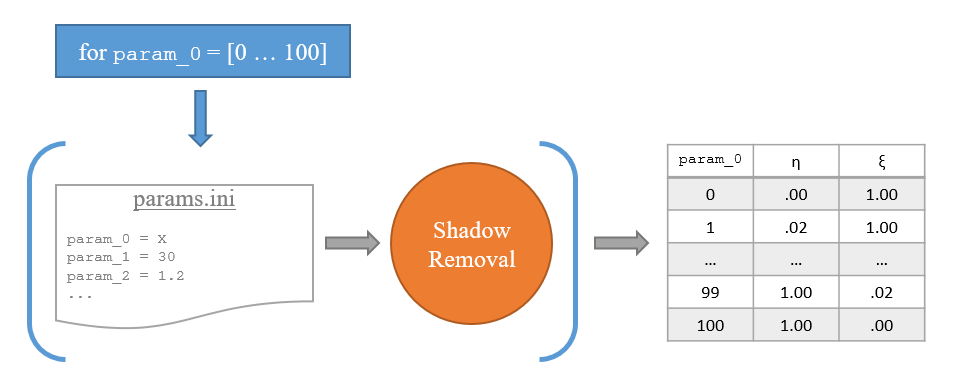
\includegraphics[width=1\linewidth]{figures/gui_iterate.png}
  \caption{For one frame, a parameter is systematically iterated to provide detection/discrimination results for each possible parameter value.}
  \label{fig:guiiterate}
\end{figure}

\begin{figure}
  \centering
  \begin{subfigure}{1\linewidth}
  	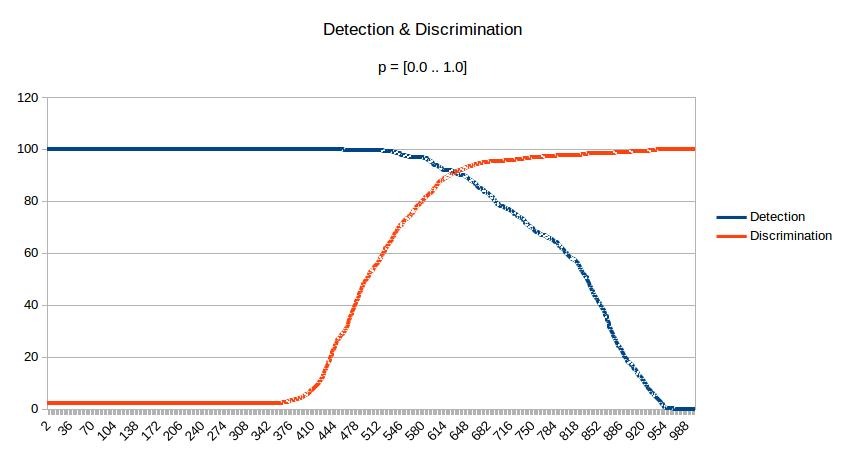
\includegraphics[width=1\linewidth]{figures/campus_dd.jpg}
  \caption{Detection (blue) and Discrimination (orange) rates are charted against the iterated parameter value (x-axis).}
  \end{subfigure}
  \hfill
  \begin{subfigure}{1\linewidth}
  	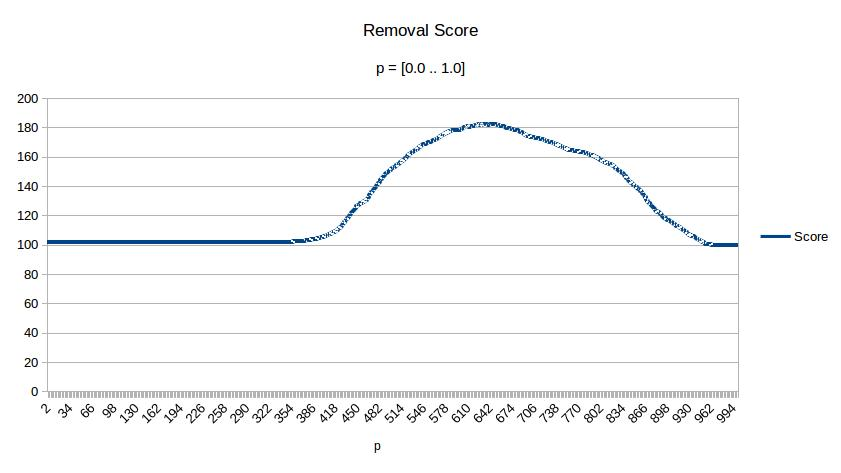
\includegraphics[width=1\linewidth]{figures/campus_score.jpg}
  \caption{For each parameter value, detection and discrimination are summed to produce a score. The global maximum of this value is the optimal parameter value ($pr$*).}
  \end{subfigure}
\caption{}
\label{fig:campusddscore}
\end{figure}

\hl{We also utilize the iterative process to determine the optimal value of $pr$ for each frame in a dataset, i.e., which $pr$ value yields the greatest improvements in detection and discrimination. This optimal value is denoted as $pr$*. The detection and discrimination rates calculated are summed, resulting in a shadow removal score $\Xi(pr)$ (Eqn. \ref{eqn:score}), which quantifies the efficacy of the shadow removal algorithm given a certain $pr$ value. Figure \ref{fig:campusddscore}(b) illustrates the score calculated using the responses found in Figure \ref{fig:campusddscore}(a). We define the optimal value $pr$* as the global maximum of $\Xi(pr)$ (Eqn. \ref{eqn:optscore}).}

\begin{equation}
\Xi(pr) = \eta(pr) + \xi(pr)
\label{eqn:score}
\end{equation}

\begin{equation}
pr\emph{*} = \Xi\emph{*}(pr)
\end{equation}

\hl{To assess the performance of algorithms throughout a dataset, $pr$* is calculated for each frame. The $pr$* values are used to determine degrees of correlation for an environment, and set the foundation for a general model of arbitrary shadow removal improvement.}

\subsection{Algorithm Selection Strategy} \label{section:selectalgorithm}

Using the tools detailed in section \ref{section:assesstools}, we perform a brief qualitative assessment of the shadow removal algorithms' sensitivity. \hl{Given} the diversity of shadow removal methods, a wide array of environmental factors potentially may influence an even wider array of algorithmic parameters. The scope of \hl{this research} has therefore been \hl{focused on} identifying a suitable algorithm to assess, linking a parameter (\hl{intrinsic} to this algorithm) to unique environmental \hl{properties} or \hl{changes}, \hl{and developing a model for real-time parameter adaptation based on correlations found.}
%and begin the construction of a general model of shadow removal improvement given \hl{analogous} parameters.

%Identifying an appropriate algorithm for assessment means highlighting a shadow removal method that demonstrates consistently reasonable sensitivity to changes in environmental characteristics. Simultaneously, a candidate for deeper analysis must demonstrate consistency in its detection/discrimination integrity throughout most frames of a dataset, with few sizable deviations. If the study were not constrained in this manner, the motivation of this research quickly becomes redundant, as the sheer amount of interdependent variables brings the problem to levels generally reserved for unsupervised clustering and other big-data approaches. As this study means to link qualitative environmental characteristics to quantitative tangible improvement, this approach would detour research into a different realm entirely.

Candidate shadow removal algorithms \hl{are evaluated} according \hl{to the correlation between their detection and discrimination} over time, and qualitative observations attributed to a dataset; e.g., the PETS1 dataset experiences a large illumination change midway through its sampling, which is taken into account when searching for trends among the \hl{accuracy} of a candidate method. For example, Figure \ref{fig:selectinganalgorithm} charts the efficacy of each shadow removal method against the number of SIFT parameters detected in a frame.

\begin{figure}
\centering
\begin{subfigure}{.49\linewidth}
  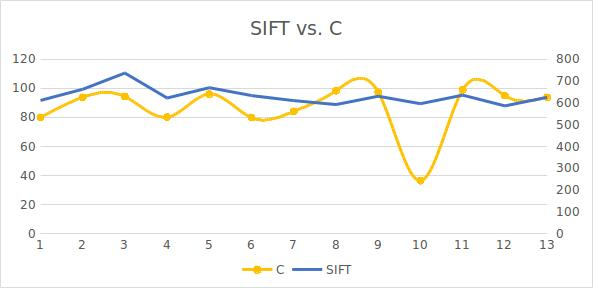
\includegraphics[width=1\linewidth]{figures/selectinganalgorithm_chromacity.jpg}
  \caption{Chromacity removal.}
\end{subfigure}
\hfill
\begin{subfigure}{.49\linewidth}
  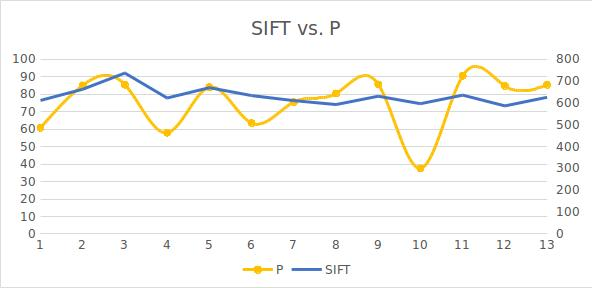
\includegraphics[width=1\linewidth]{figures/selectinganalgorithm_physical.jpg}
  \caption{Physical removal.}
\end{subfigure}
\hfill
\begin{subfigure}{.49\linewidth}
  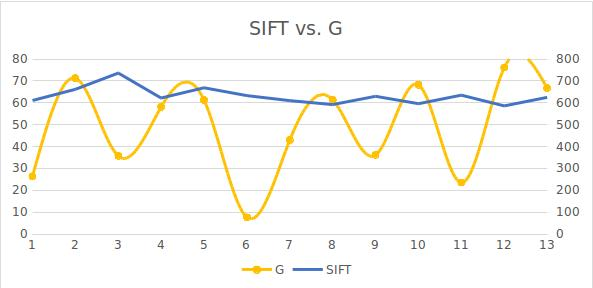
\includegraphics[width=1\linewidth]{figures/selectinganalgorithm_geometry.jpg}
  \caption{Geometry removal.}
\end{subfigure}
\hfill
\begin{subfigure}{.49\linewidth}
  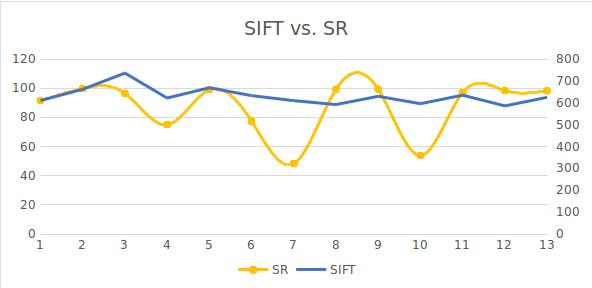
\includegraphics[width=1\linewidth]{figures/selectinganalgorithm_srt.jpg}
  \caption{Small-Region Texture removal.}
\end{subfigure}
\hfill
\begin{subfigure}{.49\linewidth}
  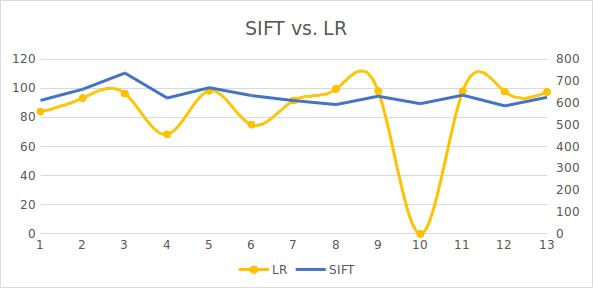
\includegraphics[width=1\linewidth]{figures/selectinganalgorithm_lrt.jpg}
  \caption{Large-Region Texture removal.}
\end{subfigure}

\caption{Shadow removal methods and their performance v. number of detected SIFT features in an image (aton\_hallway).}
\label{fig:selectinganalgorithm}
\end{figure}

\subsubsection{Evaluation of Methods}

\hl{We evaluate popular shadow removal methods introduced in section \ref{section:removalmethods}: Chromacity, Physical, Geometry, SRT, and LRT. This section describes our rationale for using Physical shadow removal as part of our proof-of-concept, implemented starting in section \ref{section:selectparameter}. Our evaluation considers the tunable parameters of an algorithm, dependence on environmental properties and content, and sensitivity of relevant parameters.}

A parameter's sensitivity is evaluated by viewing its detection and discrimination responses ($\eta(pr)$, $\xi(pr)$). Figure \ref{fig:paramsensitivity} illustrates what is considered a sensitive parameter. A parameter is considered sensitive when a narrow range of parameter values affect detection and discrimination rates disproportionately. This sensitivity causes problems for an adaptive model, as the range of potential optimal parameter values ($pr$*) is too small to correlate with environmental properties. 

\begin{figure}
\centering
\begin{subfigure}{.49\linewidth}
  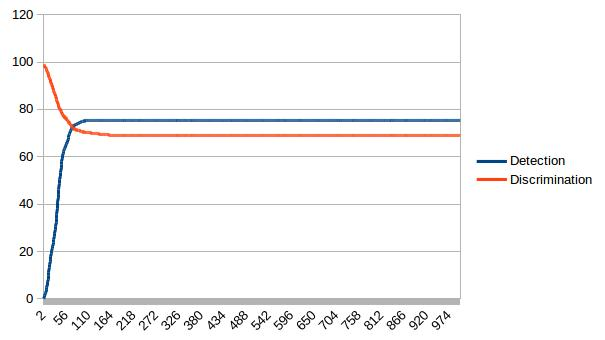
\includegraphics[width=1\linewidth]{figures/sensitive_param.jpg}
  \caption{}
\end{subfigure}
\hfill
\begin{subfigure}{.49\linewidth}
  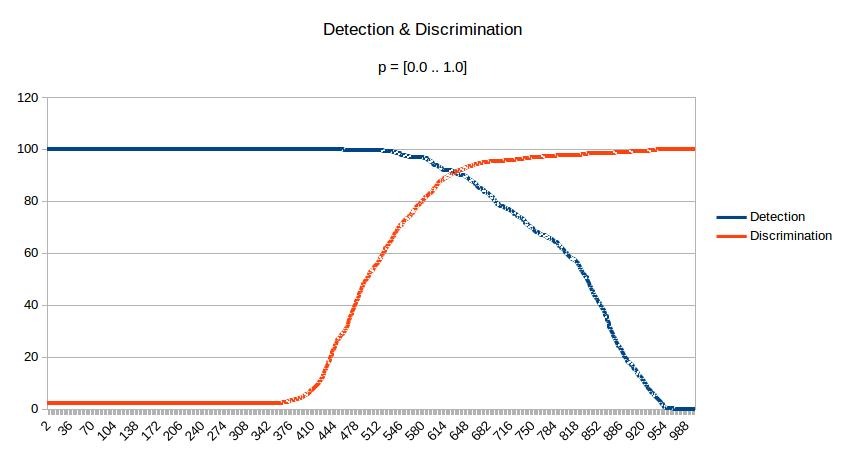
\includegraphics[width=1\linewidth]{figures/campus_dd.jpg}
  \caption{}
\end{subfigure}

\caption{(a) depicts a sensitive parameter, while (b) represents a typical parameter.}
\label{fig:paramsensitivity}
\end{figure}

%Both Geometry removal and SRT removal were shown to behave highly erratically from frame to frame \hl{even} within an environmentally consistent dataset. Geometry-based removal remains dependent on the shape and consistency of processed foreground objects, \hl{and therefore} dependent on the consistency of whichever foreground extractor is used for a scene. \hl{This dependency is not related to the properties of shadows within an environment, therefore we do not pursue further analysis with Geometry removal}. SRT removal is based upon a series of Gabor filters used to characterize textural patches found in shadows, and match them to a corresponding background model. This technique requires that shadows cover textural portions of the background model large enough to perform meaningful analysis. The algorithm carries with it no meaningful contingencies for this limitation. The parameters associated with SRT removal define little avenue for improvement of shadow removal in most cases, and defines no avenue for cases mentioned where the shadows are too small. This dependence on a shadow's area, coupled with no parameters suitable to improve detection, eliminated SRT removal from candidacy. 

Both Geometry removal and SRT removal were shown to behave highly erratically from frame to frame \hl{even} within an environmentally consistent dataset, \hl{demonstrated in Figure \ref{fig:geosrterratic}}. Geometry-based removal remains dependent on the shape and consistency of processed foreground objects, \hl{and therefore} dependent on the consistency of whichever foreground extractor is used for a scene. \hl{Furthermore, the algorithmic parameters associated with Geometry removal apply only to scenes in which the previous dependency is already fulfilled, i.e., the tunable parameters are relevant only to the geometric shapes necessary to enable Geometry removal.} \hl{These dependencies are not related to the properties of shadows within an environment, therefore we do not pursue further analysis with Geometry removal}. SRT removal is based upon a series of Gabor filters used to characterize textural patches found in shadows, and match them to a corresponding background model. This technique requires that shadows cover textural portions of the background model large enough to perform meaningful analysis. Manual tuning of SRT's algorithmic parameters provides no benefit to the algorithms detection or discrimination rates. This dependence on a shadow's area, coupled with the lack of parameters suitable to improve \hl{shadow removal}, eliminated SRT removal from candidacy. 

\begin{sidewaysfigure}
\centering
\begin{subfigure}{.49\linewidth}
  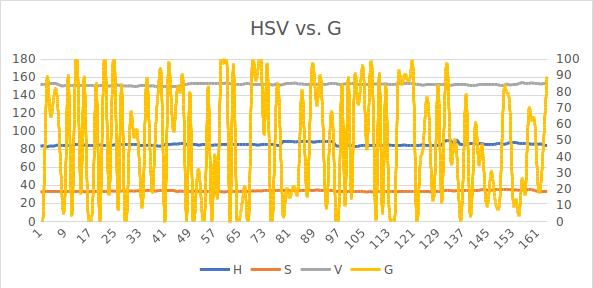
\includegraphics[width=1\linewidth]{figures/caviar_geo_erratic.jpg}
  \caption{Geometry}
\end{subfigure}
\hfill
\begin{subfigure}{.49\linewidth}
  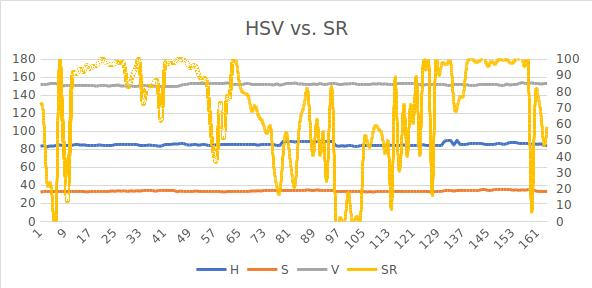
\includegraphics[width=1\linewidth]{figures/caviar_srt_erratic.jpg}
  \caption{SRT}
\end{subfigure}
\hfill
\begin{subfigure}{.49\linewidth}
  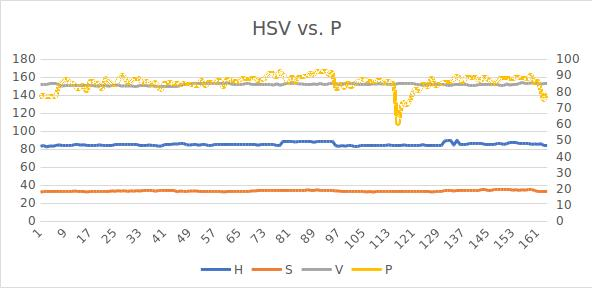
\includegraphics[width=1\linewidth]{figures/caviar_phys_calm.jpg}
  \caption{Physical}
\end{subfigure}
\hfill
\begin{subfigure}{.49\linewidth}
  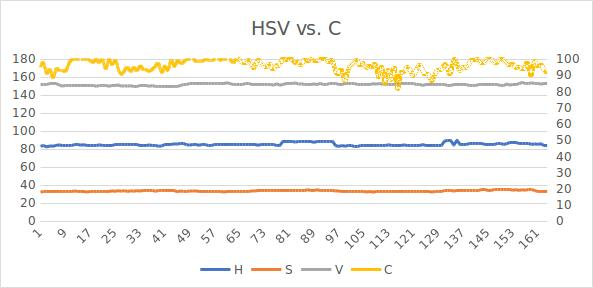
\includegraphics[width=1\linewidth]{figures/caviar_chrom_calm.jpg}
  \caption{Chromacity}
\end{subfigure}

\caption{(a) and (b) showcase erratic shadow detection, compared to (c) and (d) using the same frames.}
\label{fig:geosrterratic}
\end{sidewaysfigure}

%Sanin et al.'s Large-Region Texture algorithm was also eliminated from the assessment due to its temperamental inter-frame performance, similar to the methods above. Some environments, such as the roadways of aton\_highway3, yielded null detections for all frames \textbf{NOTE: This specific test needs to be rerun, I know why the NULLs happened. Everything else is fine though}. The Large-Region Texture algorithm recognizes the pitfalls of the Small-Region approach, such as overly-small texture regions, and attempts to correct them using hard-coded parameters. Unfortunately, the algorithm as a whole displays an overly large sensitivity to change, both inter and intra-dataset (see Figure \ref{fig:lrt_sensitivity}). In a larger scoped study, one may approach this algorithm as an ideal candidate for potential improvement, given its large swath of tunable parameters and variable responses. However, for those reasons it was excluded from the remainder of this study. By selecting an algorithm with more controlled responses to change of environment, we can extend insights gleaned into improvements for other algorithms, including this one.

Sanin et al.'s Large-Region Texture algorithm was also eliminated from the assessment due to its \hl{inconsistent shadow removal}, similar to Geometry and SRT removal (Figure \ref{fig:lr_sensitivity}). Some environments, such as the roadways of aton\_highway1, yielded null detections for all frames. The Large-Region Texture algorithm recognizes the pitfalls of the Small-Region approach, such as restrictive texture regions, and attempts to correct them using hard-coded parameters. \hl{The algorithm primarily displays a sensitivity to environment, as identical parameter values produce vastly disparate shadow removal performances (Figure \ref{fig:lr_sensitivity}). LRT also demonstrates varying levels of parametric sensitivity, also dependent on the deployment environment. For example, in environments such as aton\_campus and aton\_hallway, the parameter \textit{avgAttenThresh} is highly sensitive, similar to Figure \ref{fig:paramsensitivity}(a); however, when deployed in aton\_highway1, \textit{avgAttenThresh} does not affect detection or discrimination for any value.}

\begin{figure}
\centering
\begin{subfigure}{.8\linewidth}
  \centering
  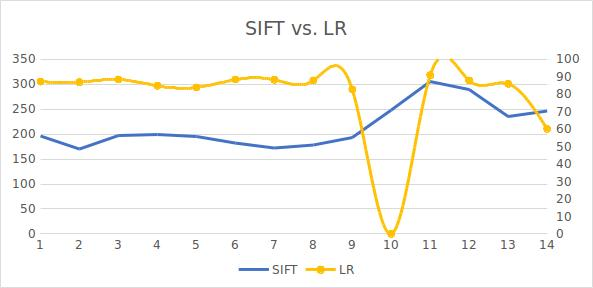
\includegraphics[width=1\linewidth]{figures/lrt_sensitivity_2.jpg}
  \caption{}
  \label{fig:sub1}
\end{subfigure}
\hfill
\begin{subfigure}{.8\linewidth}
  \centering
  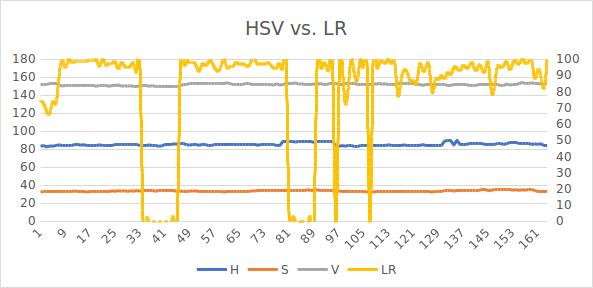
\includegraphics[width=1\linewidth]{figures/lrt_sensitivity_1.jpg}
  \caption{}
  \label{fig:sub2}
\end{subfigure}
\caption{(a) displays the consistent nature of LRT in some environments, while (b) demonstrates erratic dips in consistency.}
\label{fig:lrt_sensitivity}
\end{figure}

%Finally, both Chromacity-based and Physical-based shadow removal held the qualities ascribed to a suitable algorithm for exploration. In both cases, trends are observed, consistency of detection is within reasonable range, and the modification of parameters produces a scalable and easily observable response. This is visualized in Figure \ref{fig:similarities}.

\begin{figure}
\centering
\begin{subfigure}{.49\linewidth}
  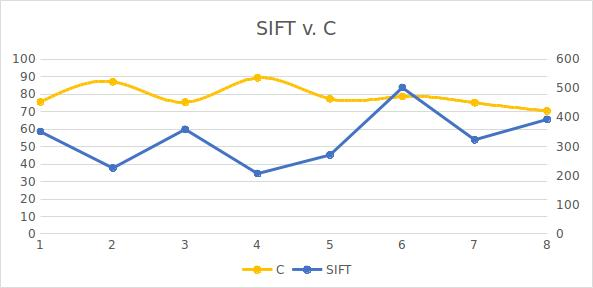
\includegraphics[width=1\linewidth]{figures/similarities_chromacity_highway1.jpg}
\end{subfigure}
\hfill
\begin{subfigure}{.49\linewidth}
  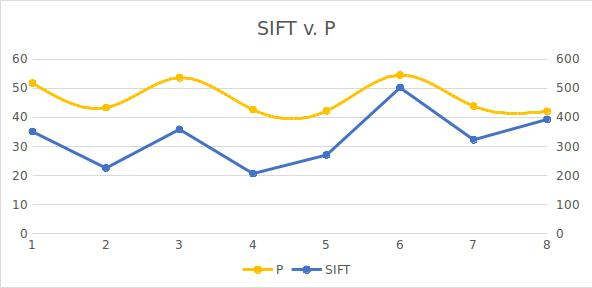
\includegraphics[width=1\linewidth]{figures/similarities_physical_highway1.jpg}

\end{subfigure}
\hfill
\begin{subfigure}{.49\linewidth}
  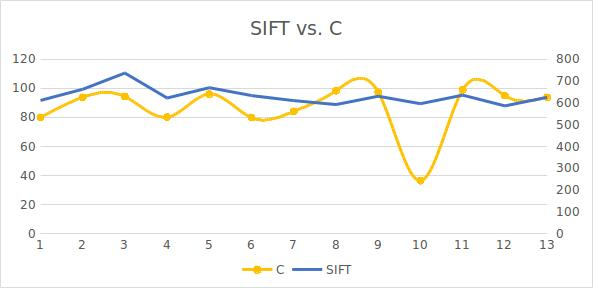
\includegraphics[width=1\linewidth]{figures/similarities_chromacity_hallway.jpg}
  \caption{Chromacity}
\end{subfigure}
\hfill
\begin{subfigure}{.49\linewidth}
  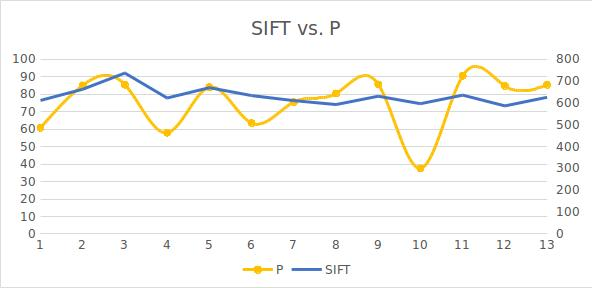
\includegraphics[width=1\linewidth]{figures/similarities_physical_hallway.jpg}
  \caption{Physical}
\end{subfigure}

\caption{Chromacity (a) and Physical (b) shadow removal demonstrate similar responses to multiple datasets.}
\label{fig:similarities}
\end{figure}

\hl{Chromacity and Physical shadow removal provide tunable parameters that lie within acceptable ranges of sensitivity. An example of an acceptable range of sensitivity is seen in Figure \ref{fig:paramsensitivity}(b). Chromacity and Physical shadow removal also display consistency between datasets, i.e., none of the datasets provided particularly poor results that are not linked to an environmental property change, such as illumination change. The Chromacity removal algorithm succeeds due to the tendency of shadows (within a dataset) to remain a consistent darkness when compared to the corresponding background model. However, this simple approach can prove problematic when illumination changes occur within a dataset. Physical shadow removal utilizes a similar system of gauging a shadow's darkness compared to a background model - what is referred to as a weak detector [\ref{Phys, Chroma, LRT}] - and implicitly suffers similar breakdowns of detection when presented with significant illumination flux within a dataset. Although they both suffer, Physical shadow removal employs a strong detector [\ref{things}] to increase detection and discrimination at the cost of processing time. In the end, Physical shadow removal was selected as the main experimental framework for this study, triumphing over Chromacity shadow removal in part due to its more sophisticated model.}

\subsection{Selecting a Parameter - Physical Shadow Removal} \label{section:selectparameter}

Physical shadow removal operates in two stages: the weak detector, and the strong detector. The weak detector typically identifies candidate shadow pixels simply by eliminating impossible pixels, i.e., pixels that are brighter than the background model. These candidate pixels are then provided to the strong detector, which characterizes these pixels as either shadow or foreground. Our assessment of algorithmic parameters explores parameters in both of these detector spaces. Before we can illustrate which parameters were considered for experimentation, we must first understand the parameters' place within the algorithm.

\subsubsection{Weak Detector - Physical Shadow Removal}

The purpose of the weak detector is to eliminate impossible pixels from being fed to the strong detector. The weak detector in Physical shadow removal functions similarly to the Chromacity shadow removal process; the candidate pixel is evaluated by its distance from a corresponding background pixel and sorted accordingly. The weak detector is visually, and technically, a cone projected in an RGB plane indicating the range in which a normalized shadow pixel may lie \hl{with} respect to a background model. Normalizing the shadow pixel's position relative to the background model is accomplished by computing the angular distance between the RGB vector of the foreground and the RGB vector of the background. The resultant represents the color-space deviation from foreground to background. This threshold parameter is named \textit{coneAngle} within the Physical shadow removal algorithm. The cone represents two dimensions: color deviation, and intensity (or brightness) deviation. \hl{A foreground pixel is considered a possible shadow if the normalized ratio of foreground to background brightness (scaled by a function of the color deviation) is within a pre-defined brightness range.} The tolerable brightness range, delimited by parameters named \textit{coneR1} (minimum) and \textit{coneR2} (maximum), is hard-coded within the original algorithm to be 0.3 to 1.0. This range is the maximum and minimum that the normalized ratio of foreground to background (multiplied against the cosine of the color deviation) can exist within and still be considered a possible shadow (awkward). \hl{[\ref{Physical}] illustrates the conic model in Figure \ref{fig:cone_physical}.}

\begin{figure}
  \centering
  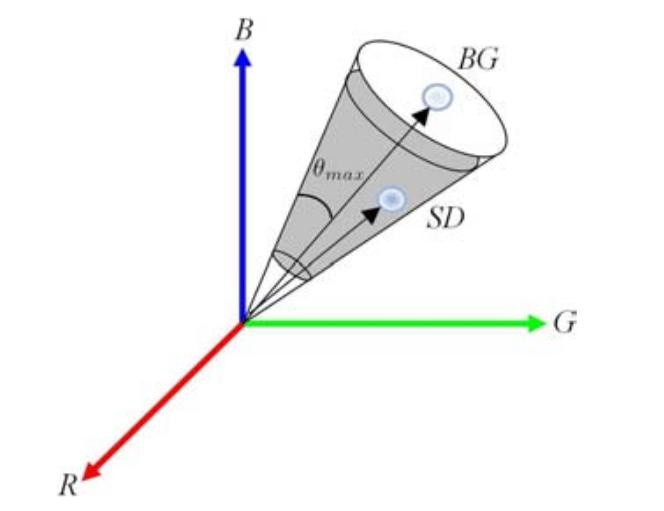
\includegraphics[width=.7\linewidth]{figures/cone_physical.jpg}
  \caption{The conical volume describing the tolerable brightness range of a shadow pixel in relation to a its illuminated counterpart.}
  \label{fig:cone_physical}
\end{figure}

The main components of the weak detector are parameterized within the algorithm to fit a general model; \textit{coneR1} $<$ $x$ $<$ \textit{coneR2} as an intensity range works reasonably well for many scenes, but there exists an optimal range for any given environment. Similarly, the maximal color angle between foreground and background vectors is dependent on environmental parameters. These parameters, \textit{coneR1}, \textit{coneR2}, and \textit{coneAngle} are therefore considered when looking for correlations with environmental conditions.

\subsubsection{Strong Detector - Physical Shadow Removal}

After the weak detector removes impossible candidates for shadow pixels, a Gaussian Mixture Model (GMM) is used to learn the color features of shadow pixels when compared to background pixels. Using the remaining pixels, the GMM estimates the normalized spectral ratio for shadows in a scene, i.e., the ratio of spectral illuminants [\ref{Physical}, \ref{spectral illum}]. More information on spectral illuminants can be found in section \ref{section:nonlinearatten}. The GMM is a framework based upon Expectation Maximization and learning over time; therefore, the initial parameters presented in the algorithm have little influence over the efficacy of shadow removal. Shadow removal displayed sensitivity to only one significant parameter, \textit{postThresh}, the parameter controlling the posterior threshold. The posterior threshold is the threshold governing shadow/foreground assignment after the posterior probability of a pixel is determined via the GMM. Since the GMM adapts to its environment, modifying the posterior threshold \hl{invalidates any learning the GMM has achieved.} Correlating \textit{postThresh} to environmental parameters is not considered in this study.

\subsubsection{Evaluation of Parameters}

Due to their integral nature to both the weak and strong detectors, the following parameters are evaluated for their effect on shadow removal: \textit{coneR1}, and \textit{coneAngle}. Each parameter is shown to have a pronounced effect on shadow removal. Figure \ref{fig:coneR1_iterate} demonstrates \textit{coneR1}'s contribution to detection/discrimination across datasets.

\begin{figure}
  \begin{subfigure}{.49\linewidth}
  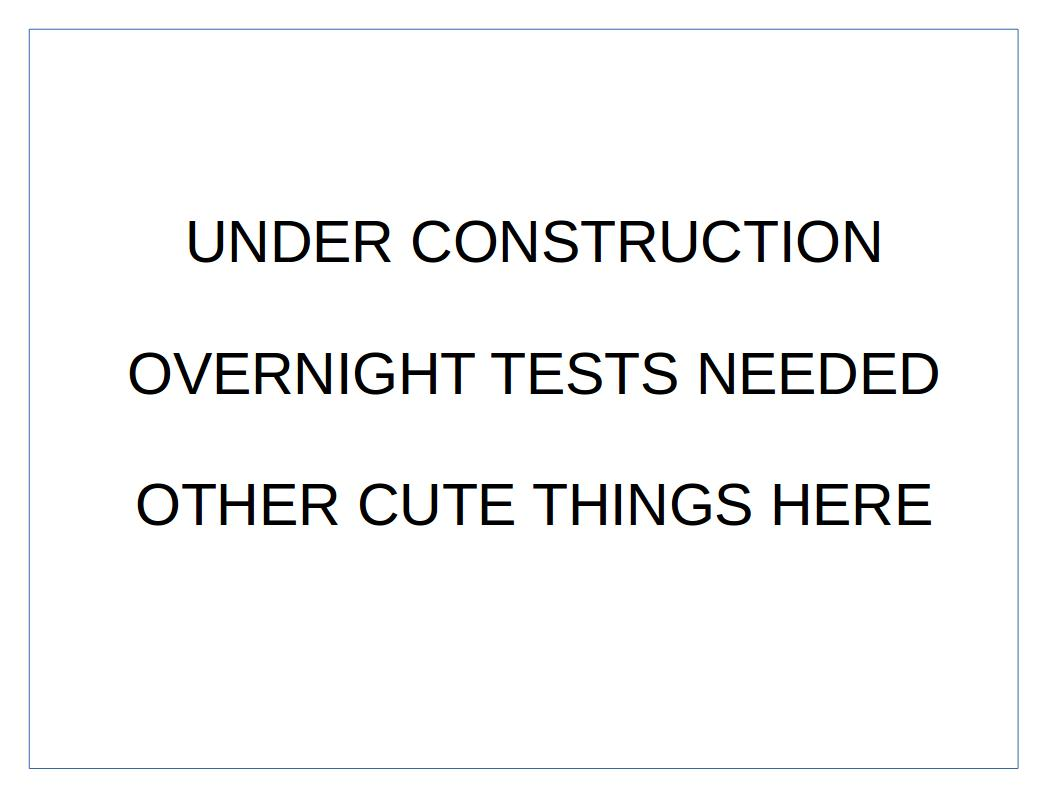
\includegraphics[width=1\linewidth]{figures/placeholder.jpg}
  \caption{}
\end{subfigure}
\hfill
\begin{subfigure}{.49\linewidth}
  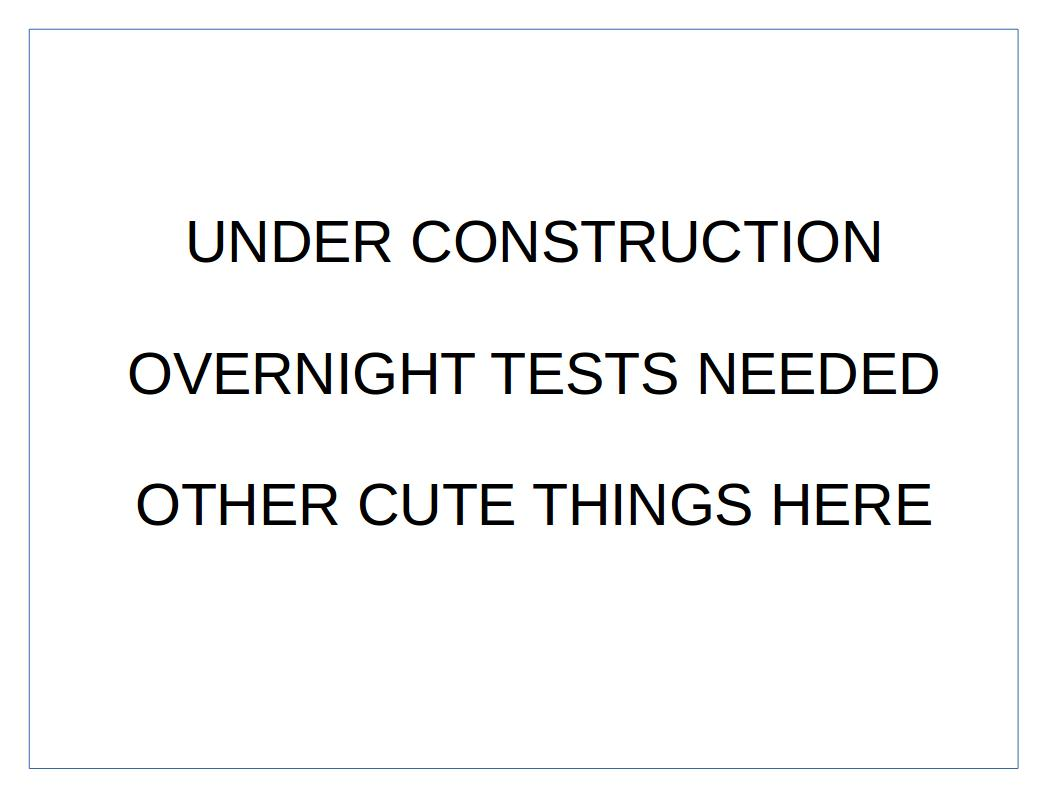
\includegraphics[width=1\linewidth]{figures/placeholder.jpg}
  \caption{}
\end{subfigure}
\hfill
\begin{subfigure}{.49\linewidth}
  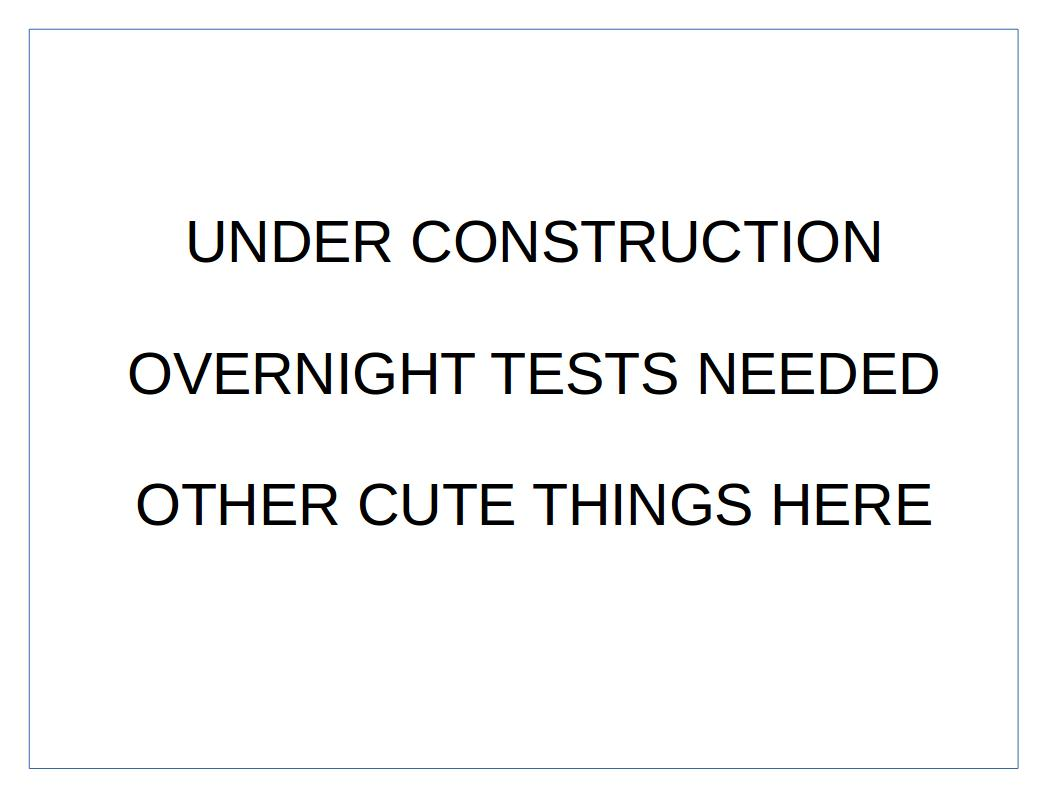
\includegraphics[width=1\linewidth]{figures/placeholder.jpg}
  \caption{}
\end{subfigure}
\hfill
\begin{subfigure}{.49\linewidth}
  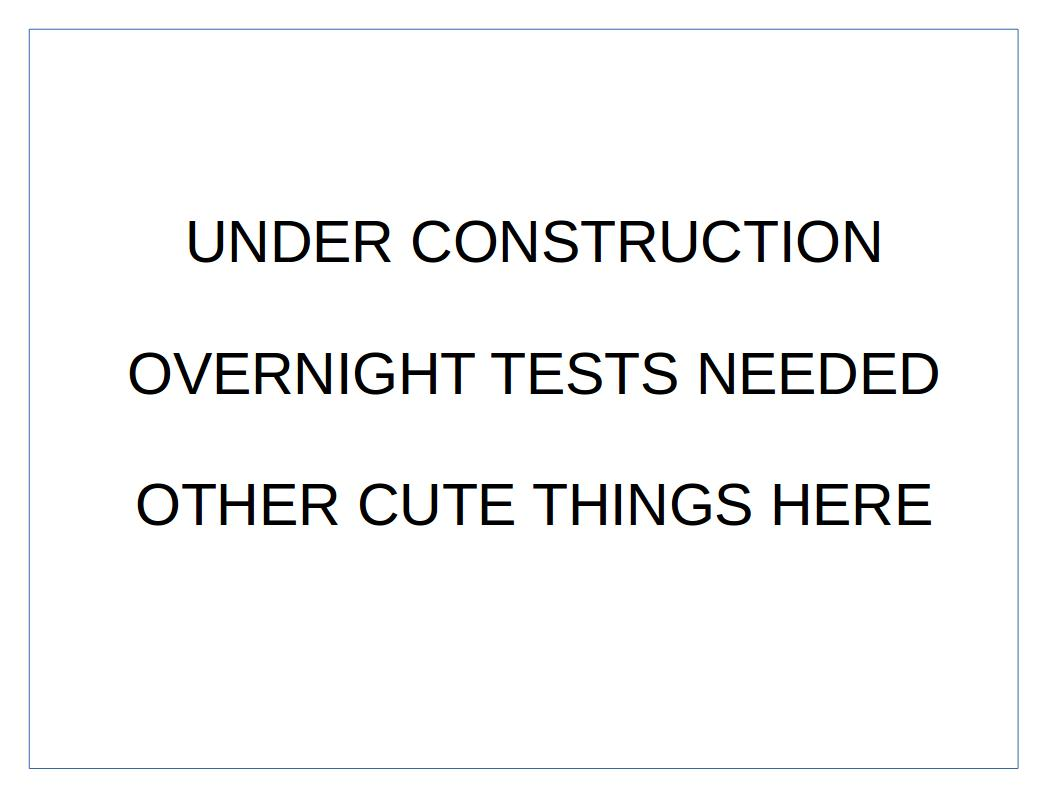
\includegraphics[width=1\linewidth]{figures/placeholder.jpg}
  \caption{}
\end{subfigure}
\hfill
\begin{subfigure}{.49\linewidth}
  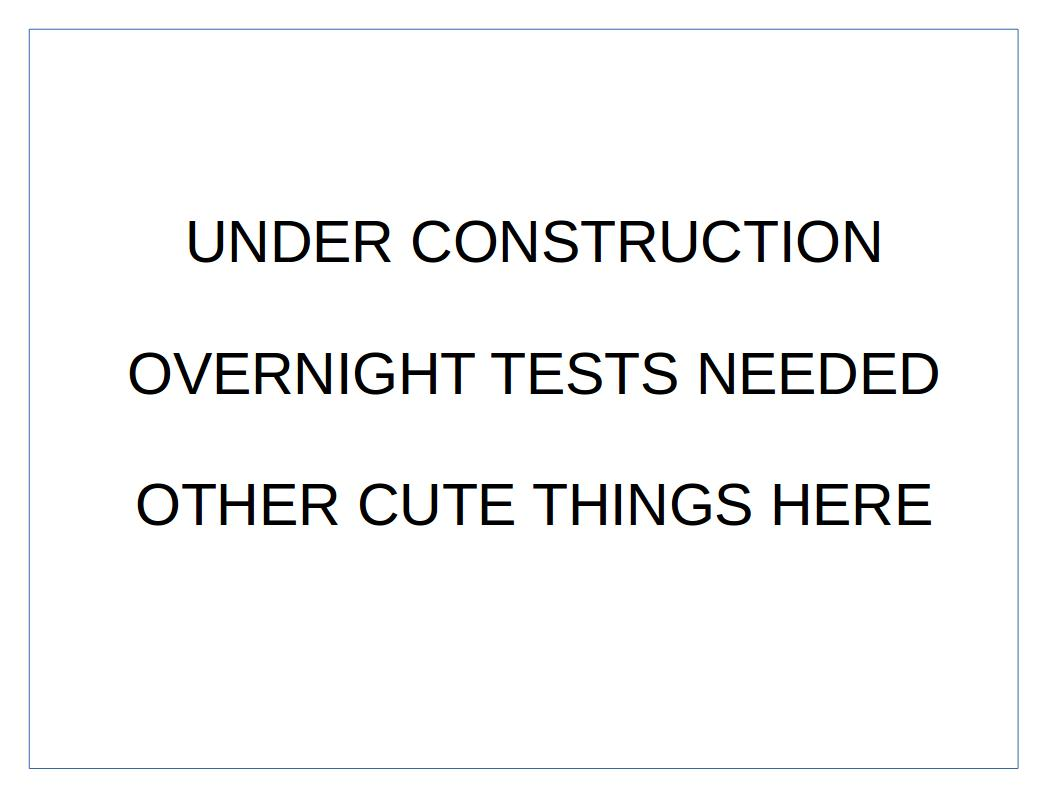
\includegraphics[width=1\linewidth]{figures/placeholder.jpg}
  \caption{}
\end{subfigure}
\hfill
\begin{subfigure}{.49\linewidth}
  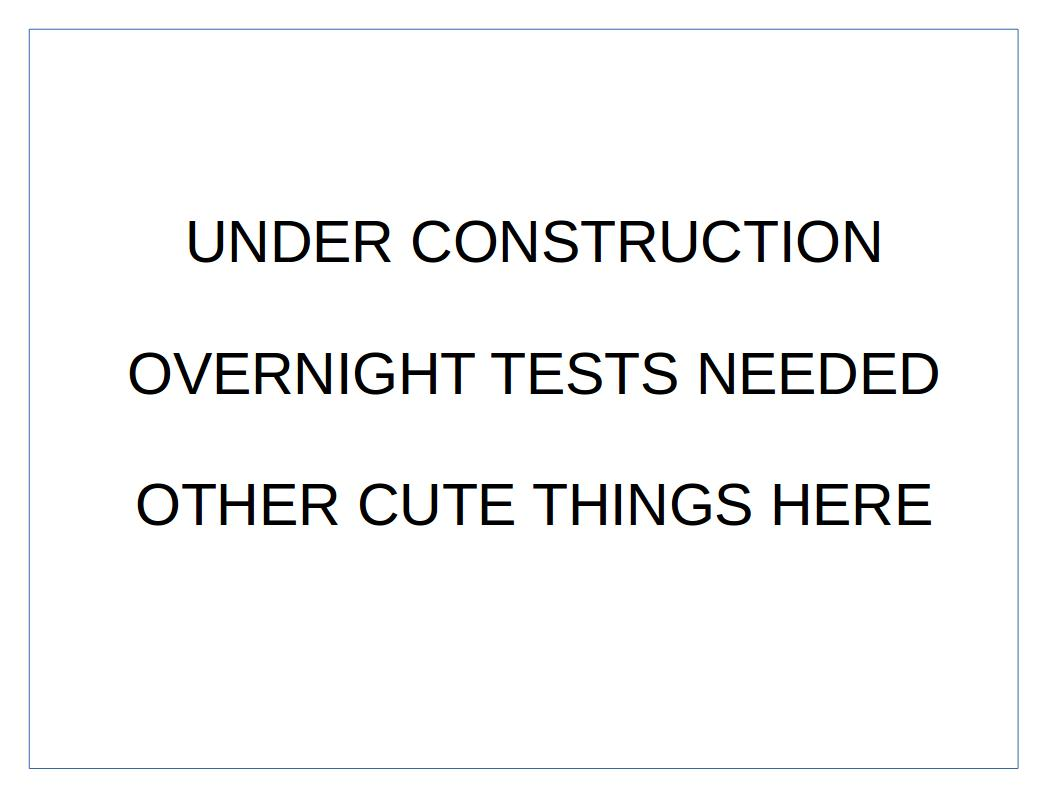
\includegraphics[width=1\linewidth]{figures/placeholder.jpg}
  \caption{}
\end{subfigure}

\caption{Detection and Discrimination rates are calculated after iteration of \textit{coneR1}. \textbf{Full results found in appendices?}}
\label{fig:coneR1_iterate}
\end{figure}

\textit{coneR1}'s effect on shadow removal remains consistent and scalable. The parameter is exercised through a large range, with an equally large range of resultant detection and discrimination rates. The wider range and relatively coarse-grained nature of the parameter allows for an easier time identifying trends and correlations with the iterations. 

\textit{coneR2} represents the upper limit of the cone around a background pixel's color representation. The parameters are inextricably tied; however, \textit{coneR2} was not subjected to as rigorous examination, as \textit{coneR2}'s dependence on the value of \textit{coneR1} creates an exponential field of possible values for each variable. 

The remaining parameters (results included in appendices) inhabit too narrow a range of sensitivity to properly exploit, e.g., \textit{coneAngle} displays erratic variation in the discovered values for optimal shadow removal, yet the optimal values are within millionths of each other. Similarly, the remaining parameters do not provide as large an improvement in shadow removal as \textit{coneR1} does. The erratic nature of the optimal parameter values, in combination with both the minimal removal improvement and \hl{narrow} range of sensitive values makes further examination of these parameters difficult. For the duration of the study, environmental feature correlations were sought after only in relation to \textit{coneR1}.

\section{Environmental Assessment - Environmental Parameters} \label{section:envassess}

\subsection{Previous Work - Large Region Texture Removal}

It is a well known phenomenon that different environmental scenes requires different algorithmic parameters (or even different algorithms) to optimally remove shadows [ref Sanin]. In Sanin's Large-Region Texture shadow removal, there are three examples of ambient scene parameters taken into account: average saturation (of foreground pixels), average attenuation (from foreground to background), and average perimeter size of foreground objects. These three global frame properties govern the value of certain algorithm parameters.

As discussed above, Large Region Texture removal is confronted with difficulties when attempting to remove shadows from regions that have small areas. In Sanin's implementation of LRT removal, average foreground perimeter is checked against a predetermined threshold. In a series of ternary statements, average perimeter informs three algorithm parameters controlling the range of area within the light/shadow border to correlate between foreground and background.

LRT removal, like Physical shadow removal, uses a weak detector to retrieve candidate shadow pixels. The candidate shadow pixels must simply fit within a certain range of Hue (H), Saturation (S), and Value (V)(or Brightness) when compared against the background model. There are two definitions of this acceptable range: $\Delta$HSV\{76,36,[0.6 - 1.0]\}, and $\Delta$HSV\{62,93,[0.21 - 0.99]\}. If the average saturation of foreground pixels exceeds a predetermined threshold, the higher values of H and S are used as the acceptable range. Similarly, if the average attenuation of the foreground pixels exceeds its threshold, the latter range of [0.21 - 0.99] is used for evaluating brightness. 

\begin{figure}
  \centering
  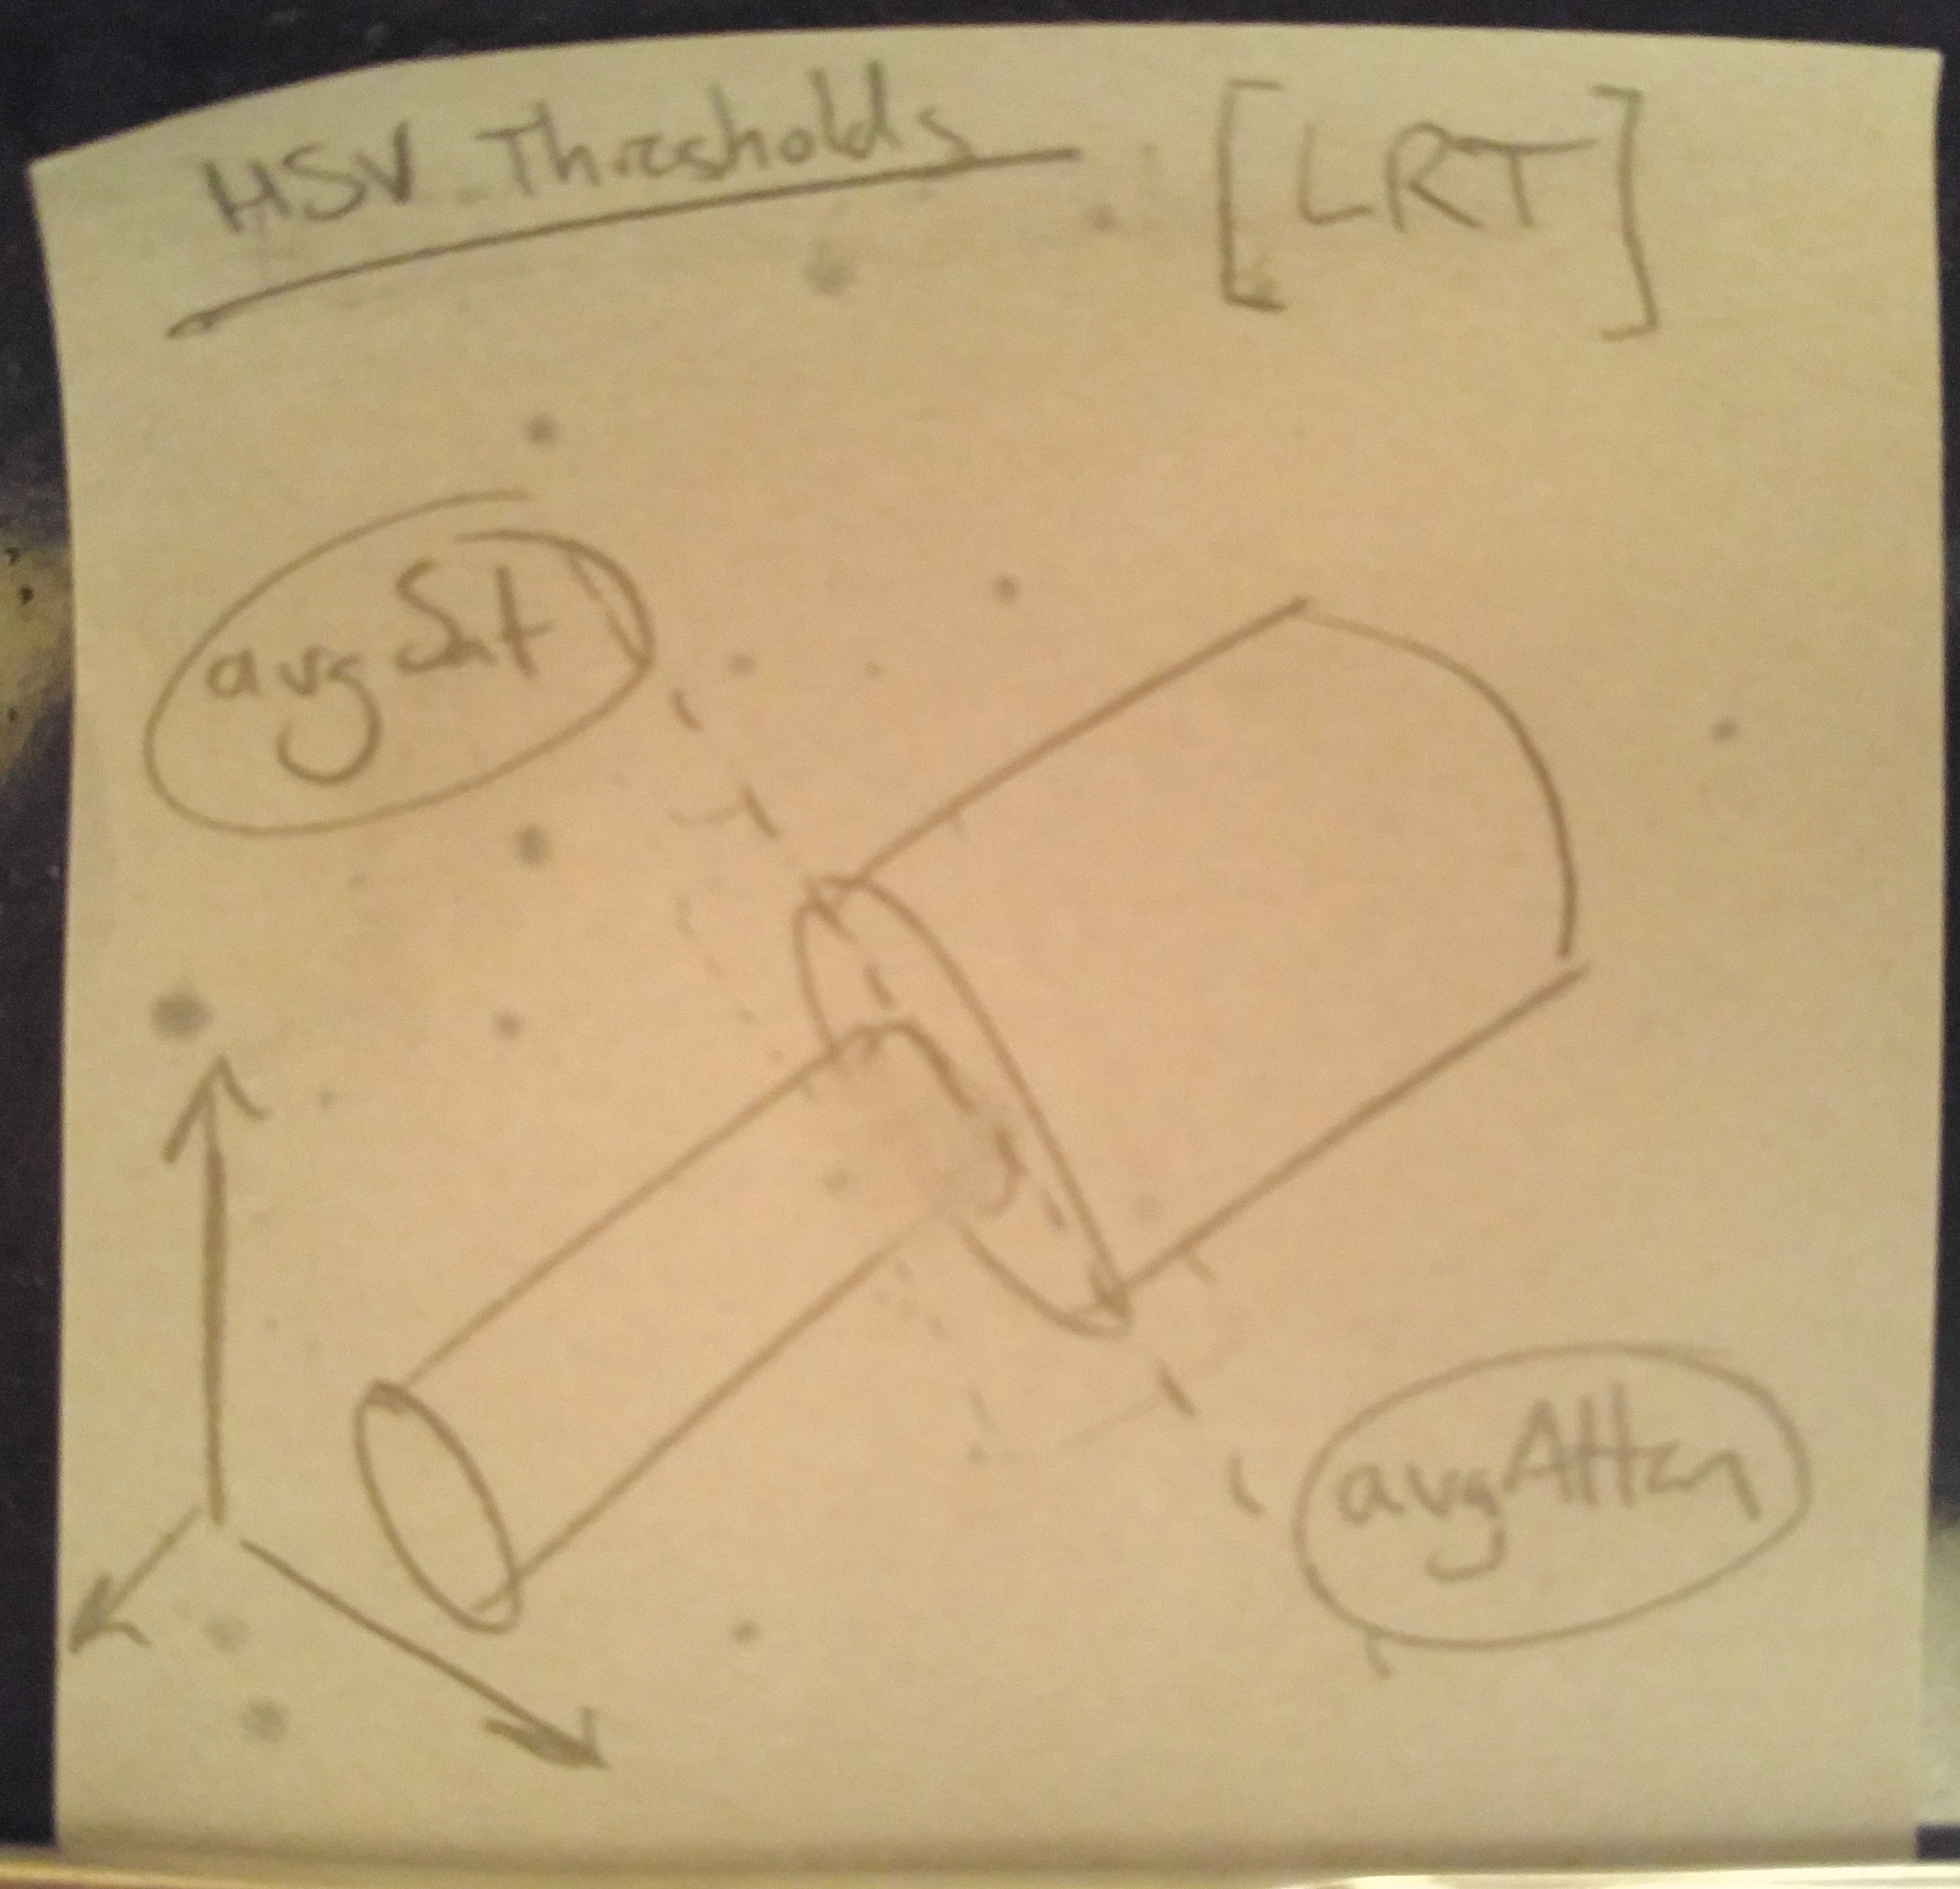
\includegraphics[width=.7\linewidth]{figures/mockup_cone_lrt.jpg}
  \caption{Visualization of the volume of constraint imposed by LRT, and how that volume changes with scene parameters \textit{average attenuation} and \textit{average saturation}.}
  \label{fig:cone_lrt}
\end{figure}

This need for adaptability underscores the motivation of this research to discover a scalable and portable solution for parameterization. In the case of Physical shadow removal, foreground object perimeter has no bearing on the efficacy of shadow removal. However, both average saturation of foreground objects and average attenuation were further scrutinized in this study.

\subsection{Attenuation and Saturation}

Attenuation represents the loss of intensity from foreground pixel to background pixel in a frame. Traditionally, brightness attenuation is represented mathematically in decibels (dB) as the ratio of background and foreground brightness.

\begin{equation}
dB = \dfrac{brightness(\vec{bg}(p))}{brightness(\vec{fg}(p))}
\end{equation}

\textit{p} represents pixel coordinates. Given this calculation method, shadow pixels trend towards attenuation values of 1.0 $<$ \textit{atten} $<$ 5.0. While this representation adheres most closely to the physical definition of light attenuation within a shadow, dB intensity loss fails to scale with known algorithm parameters. We therefore consider the reciprocal of this model ($1/dB$) of attenuation for correlation.

Alternatively, we consider the \textit{percentage change} (\%$\Delta$) model of light attenuation. This model is defined as:

\begin{equation}
\%\Delta = \dfrac{brightness(\vec{bg}(p) - \vec{fg}(p))}{brightness(\vec{bg}(p))}
\end{equation}

Similar to the dB model, $(1 - \%\Delta$) is considered for correlation, representing the percentage of a background pixel's intensity the foreground is valued at (\textbf{awkward?}).

\textbf{These attenuation calculation methods differ in the assumptions of linearity, and how it relates to shadows in an environment.}

Saturation is the measurement of 'depth of hue' in a pixel, e.g., a lower saturation means the base hue is less expressed, while a higher saturation means the color of a pixel more closely matches the base hue. The saturation level of a background pixel affects the intensity attenuation a shadow pixel experiences. While the average saturation of foreground objects can be used as a coarse guide for adjusting intensity thresholds (see LRT removal), saturation properties are used differently in this study, as seen in section \ref{section:lowcSIFT}.

\subsection{Non-linear Attenuation and Spectral Properties of Light} \label{section:nonlinearatten}

In the ideal case, the attenuation of light is an entirely linear function, i.e., a shadow pixel lies along the the vector drawn from the background pixel to the origin within the three dimensional RGB space. [re Physical]

\begin{figure}
  \centering
  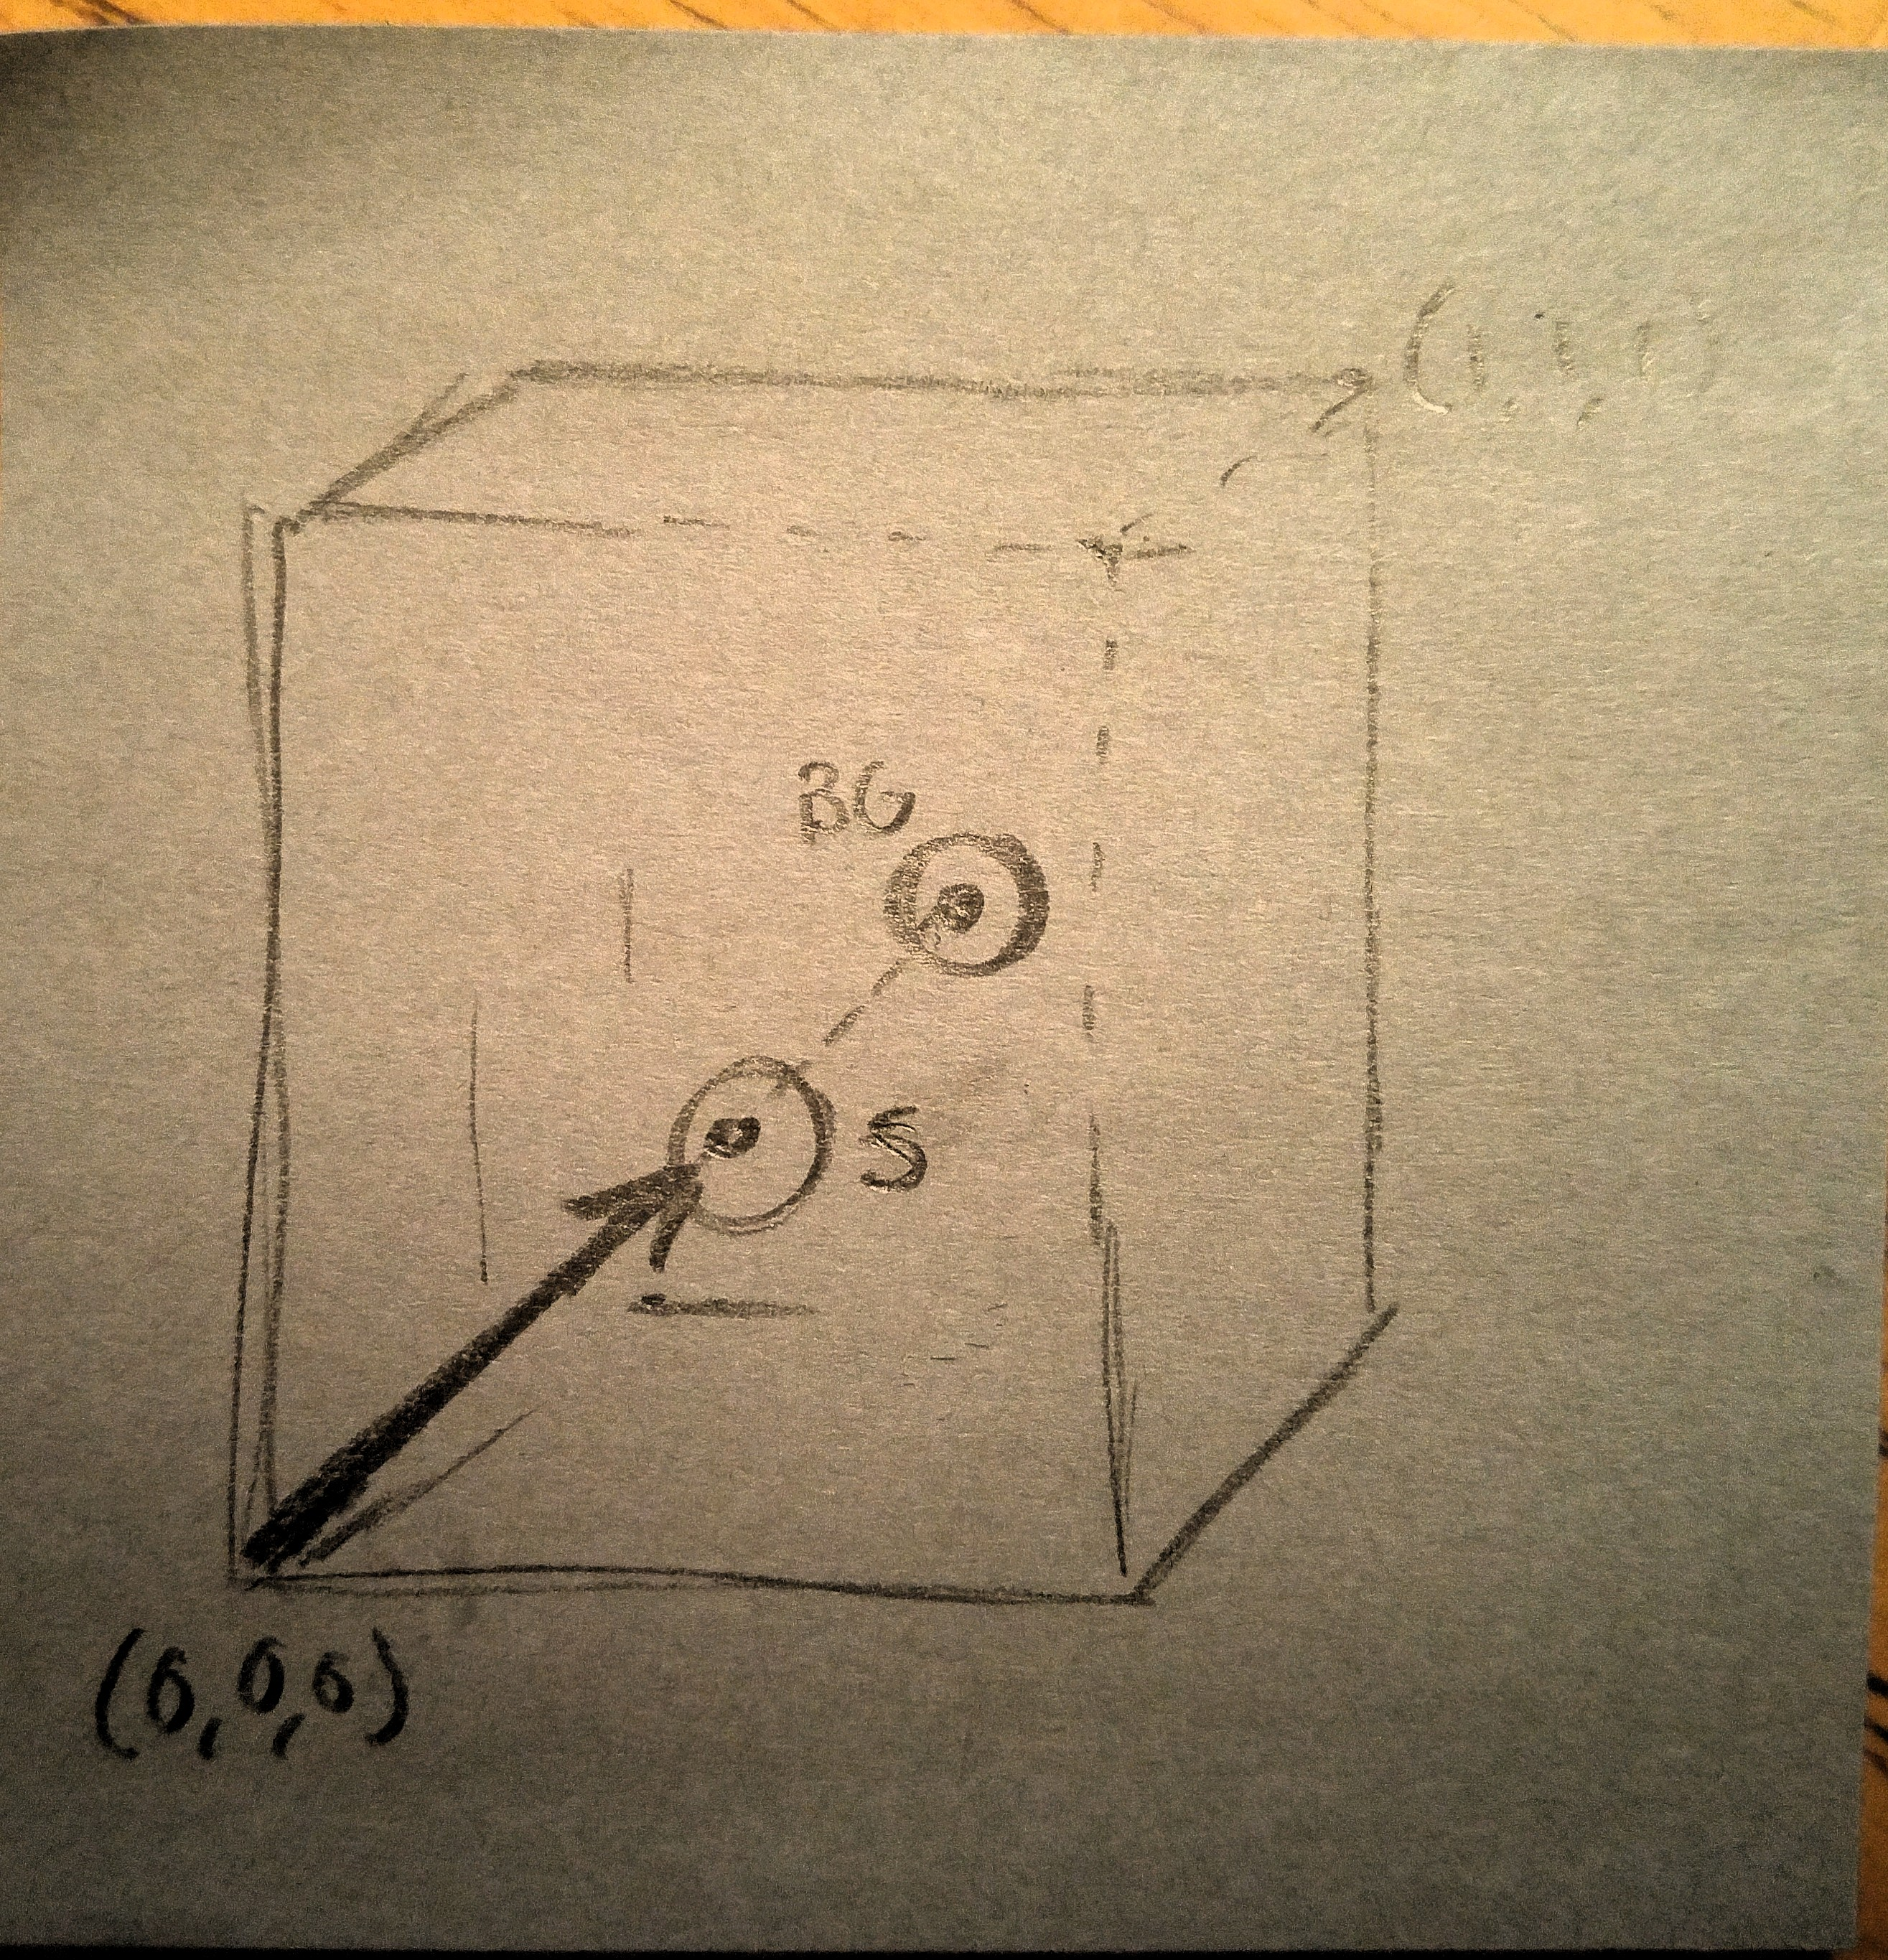
\includegraphics[width=.5\linewidth]{figures/mockup_rgbcube.jpg}
  \caption{Traditional understanding of brightness attenuation assume a shadow pixel must lie between its illuminated background model, and the origin in the RGB space.}
  \label{fig:rgbcube}
\end{figure}

Due to physical properties of illumination and reflectance, this linearity does not always hold true; cast shadows in real-world scenes commonly belong to more than one illumination source. In an outdoor scene, a shadow may be the product of direct sunlight, blue light refracted from the sky, and diffuse light scattering from nearby objects or surfaces. Any of these factors contribute to color bleed [ref phys/colorbleed], influencing the attenuation of shadow pixels. These disparate light sources are said to have different \textit{spectral power distributions}, different illumination characterized by varying concentrations of constituent wavelengths. This non-linear attenuation model is the primary motivator behind using GMM to learn a shadow's color model in [ref Phys].

\subsubsection{Observed Spectral Properties in Outdoor Scenes}

Since the spectral properties of an illumination source can not always be predicted, this study attempted to observe trends between datasets to properly characterize shadows. By visualizing the magnitude of color shift due to shadows, we can clearly partition datasets into outdoor and indoor images. Outdoor datasets experience change disproportionately in each channel of an RGB image, while indoor datasets are characterized by equal and predictable shifts in each channel.

\begin{figure}
  \centering
  \begin{subfigure}{.49\linewidth}
  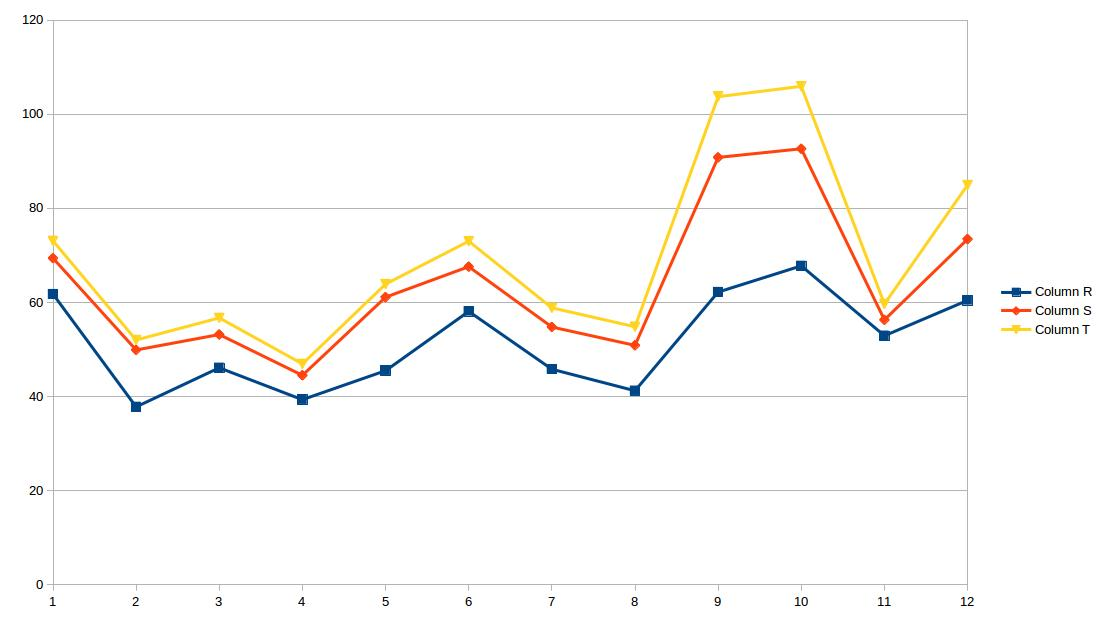
\includegraphics[width=1\linewidth]{figures/rgshift_pets1.jpg}
  \caption{PETS1}
\end{subfigure}
\hfill
\begin{subfigure}{.49\linewidth}
  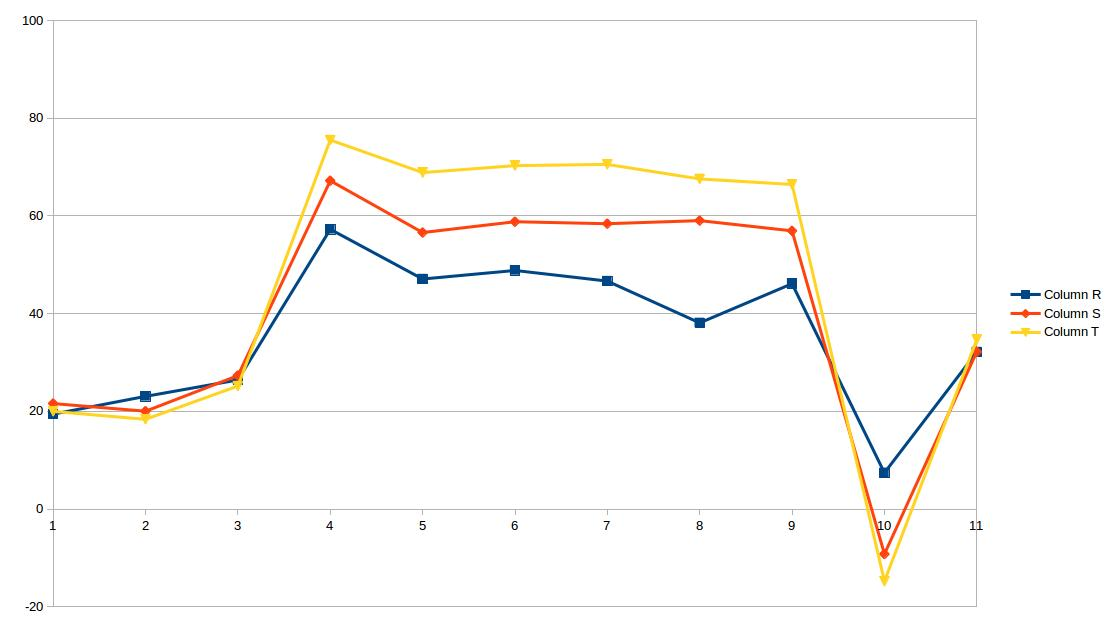
\includegraphics[width=1\linewidth]{figures/rgshift_pets2.jpg}
  \caption{PETS2}
\end{subfigure}
\hfill
\begin{subfigure}{.49\linewidth}
  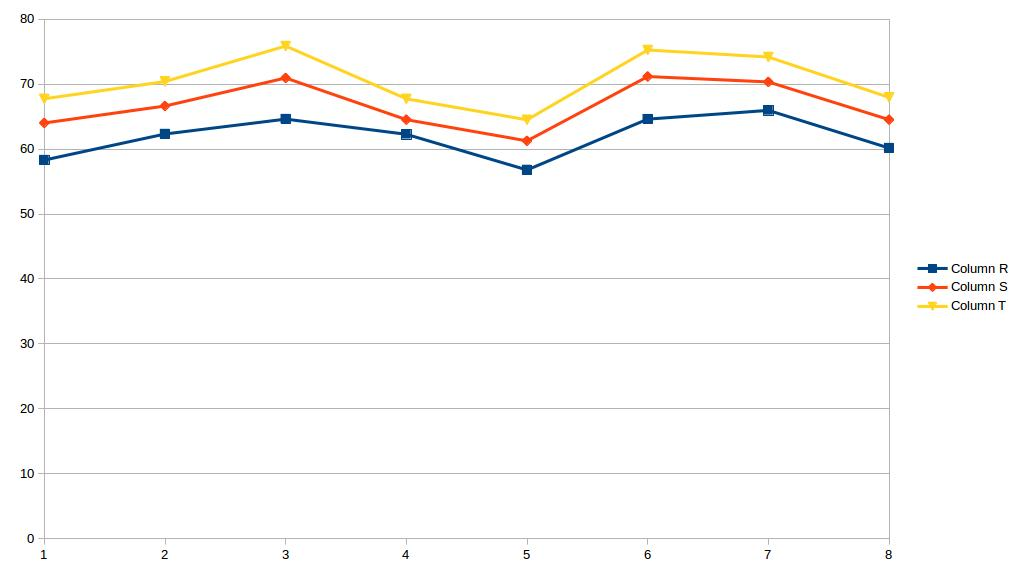
\includegraphics[width=1\linewidth]{figures/rgshift_highway1.jpg}
  \caption{aton\_highway1}
\end{subfigure}
\hfill
\begin{subfigure}{.49\linewidth}
  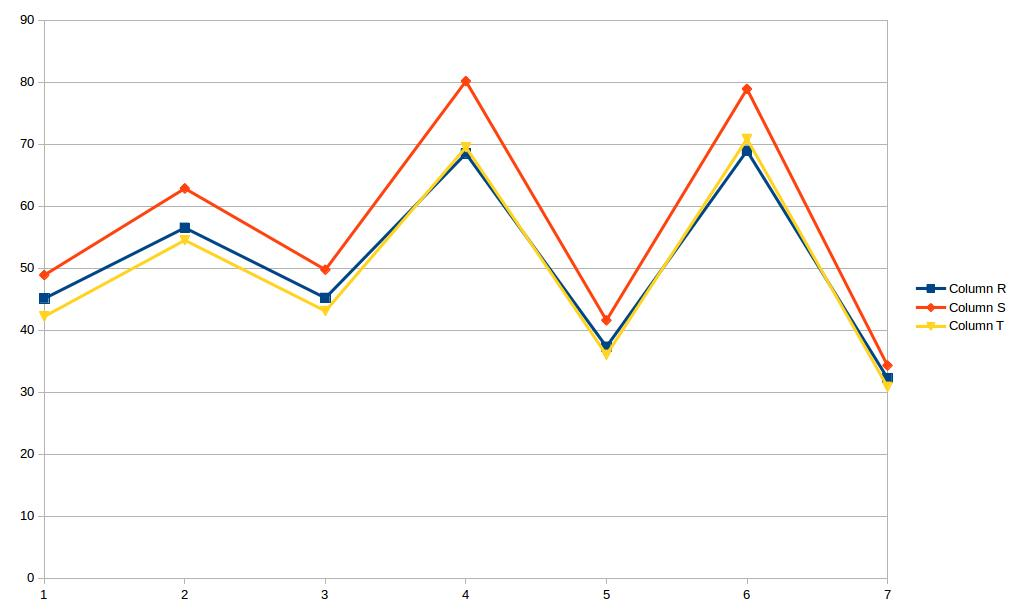
\includegraphics[width=1\linewidth]{figures/rgshift_highway3.jpg}
  \caption{aton\_highway3}
\end{subfigure}
\hfill
\begin{subfigure}{.7\linewidth}
  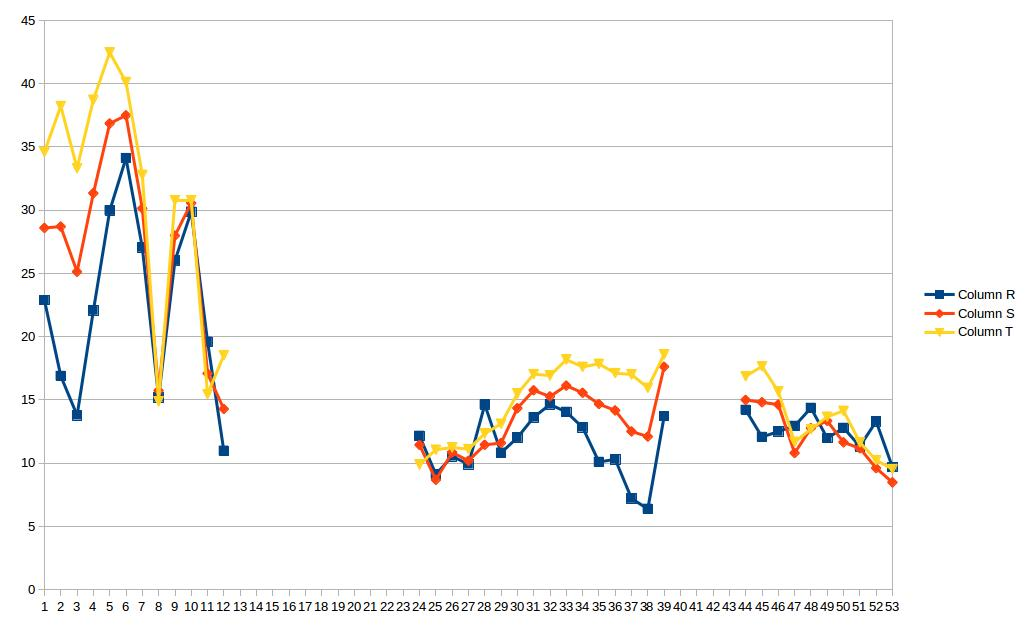
\includegraphics[width=1\linewidth]{figures/rgshift_campus.jpg}
  \caption{aton\_campus}
\end{subfigure}

\caption{Outdoor datasets demonstrate consistently greater deviations in the red and green channels. During illumination changes (evident in PETS1 and PETS2), the red and green channels shift disproportionate to that of the blue channel, indicating scattered blue light is a primary component of the shadows' spectral illuminant ratio.}
\label{fig:rgshift_outdoor}
\end{figure}

\begin{figure}
  \centering
  \begin{subfigure}{.49\linewidth}
  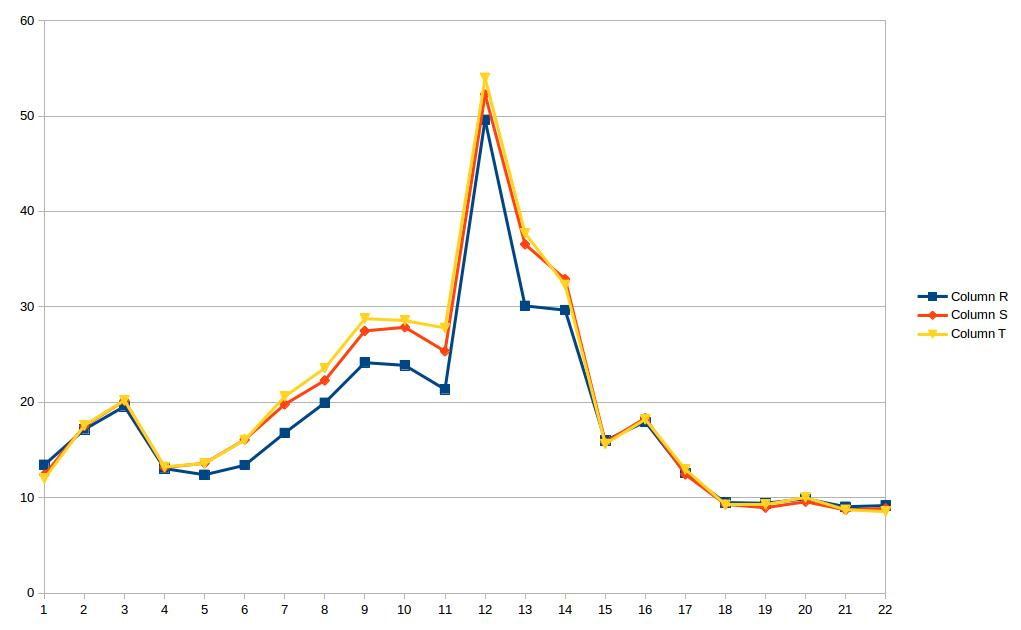
\includegraphics[width=1\linewidth]{figures/rgshift_room.jpg}
  \caption{aton\_room}
\end{subfigure}
\hfill
\begin{subfigure}{.49\linewidth}
  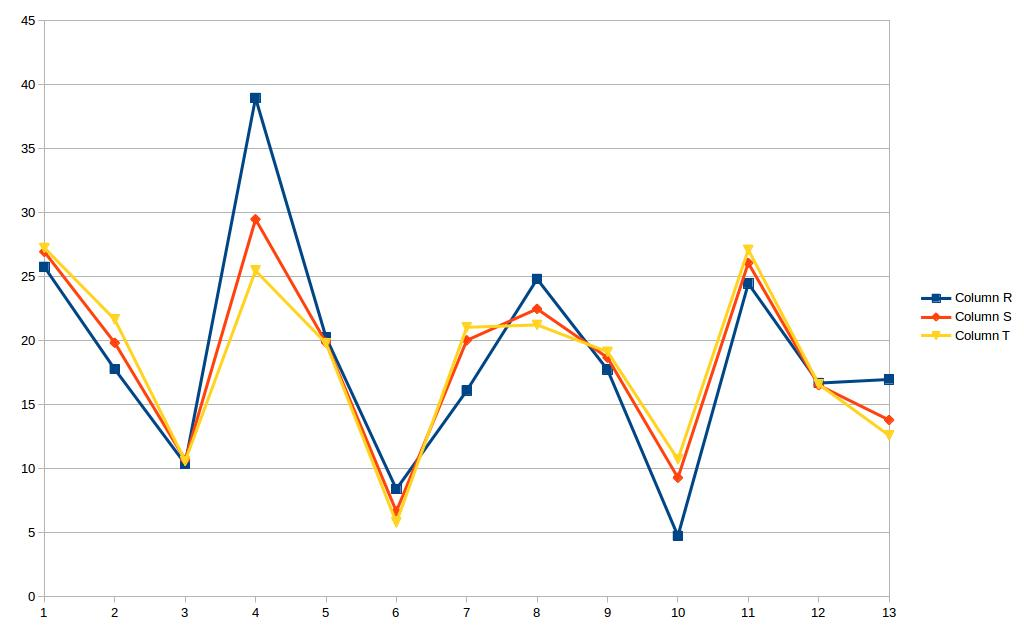
\includegraphics[width=1\linewidth]{figures/rgshift_hallway.jpg}
  \caption{aton\_hallway}
\end{subfigure}
\hfill
\begin{subfigure}{.7\linewidth}
  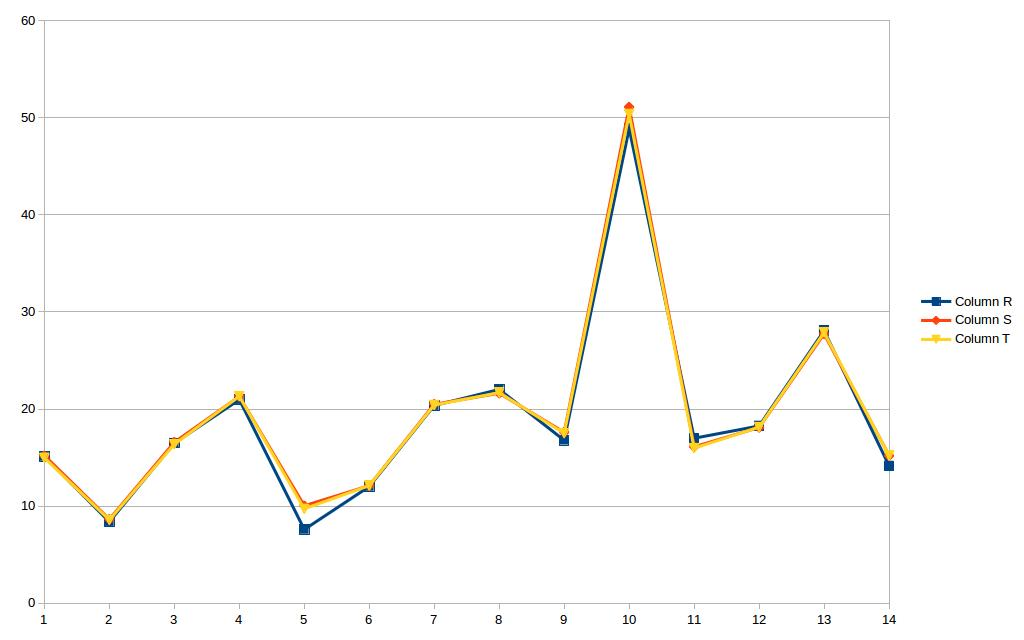
\includegraphics[width=1\linewidth]{figures/rgshift_lab.jpg}
  \caption{aton\_lab}
\end{subfigure}

\caption{Indoor datasets demonstrate closer grouping of each channel's color shift. aton\_hallway behaves most erratically of the indoor datasets. This is due to color-bleed from nearby objects, making aton\_hallway the most diverse spectral ratio of the indoor sets. aton\_lab behaves linearly, as expected.}
\label{fig:rgshift_indoor}
\end{figure}

This disproportionate discrepancy is most apparent during periods of large illumination change, found prominently in datasets PETS1 and PETS2. Examining the outdoor datasets, we can see that the red and green channels experience larger magnitude shifts that the blue channel. Based on assumed spectral power distributions of the source illumination found in the outdoor scenes, we can deduce that outdoor scenes display an introduction of blue light scattered from the sky that is not present in indoor scenes. With a spectral power distribution skewed towards blue, the red and green channels experience greater perturbation than the blue channel due to cast shadows. This study attempts to utilize this observed multi-illuminant model to better characterize the attenuation model assumed by a scene. 

\subsection{Brightness Models} \label{section:brightnessmodels}

Since attenuation is a function of brightness, understanding the myriad methods of calculating the brightness of a pixel is tantamount to accurately modeling attenuation for a scene. Similarly, in response to the spectral differences of light given the light source, the model for brightness used for a scene must adhere to what suits that scene best \textbf{awkward}. Below is a short taxonomy of popular brightness models studied. Each of the brightness models included are tested and analyzed for its affect on the average attenuation model. \textbf{NOTE: should I include hexcone/bihexcone models here?}

\subsubsection{HSV}

Also known as HSB, where Value is substituted for Brightness. Described as a 'hexcone' model, [ref hexcone HSV], brightness in an HSV representation is defined as the maximum value of the pixel represented in the red, green, and blue channels ($\vec{RGB}(p)$).

\begin{equation}
V = max(R, G, B)
\end{equation}

HSV can lead to misrepresentation of brightness as it is perceived by the human eye. This is because, as noted in Rec. 709/601 [ref 709], the same intensity of green appears brighter than that of red, which, in turn, appears brighter than the same intensity of blue. In the HSV scheme, green at full intensity ($\hat{RGB} = (0, 1, 0)$) matches the brightness of blue at full intensity ($\hat{RGB} = (0, 0, 1)$). It also minimizes contributions from channels other than the dominant channel, e.g., $\hat{RGB}(0, 1, 0)$ = $\hat{RGB}(.9, 1, .9)$. HSV therefore is best suited for environments characterized by abnormally low saturation, where light attenuation due to shadows is most linear.

\subsubsection{HSI}

HSI represents the most basic understanding of brightness, as \textit{Intensity}. 

\begin{equation}
I = \dfrac{R + G + B}{3}
\end{equation}

This understanding of brightness serves most environments properly, as it caters to each channel equally. However, HSI still suffers from the inherent luminance of certain colors, and fails to compensate for them.

\subsubsection{HSL}

HSL, a brightness A. Leone and C. Distante. Shadow detection for moving objects based on texture analysis. Pattern Recognition, 40(4):1222–1233,
2007.representation called \textit{Lightness}, is called a 'bi-hexcone' model [ref bihex] Lightness is an average of the primary and tertiary color components:

\begin{equation}
L = \dfrac{max(R,G,B) + min(R,G,B)}{2}
\end{equation}

Excluding the secondary color component has the effect of translating the brightness plane described by HSI. While perceptually similar to other brightness models, HSL provides more balanced values when one channel's value is in extrema.

\subsubsection{Relative Luminance (Y)}

Originally issued in 1982, Rec. 601 [ref?] defines 	one of the first standards for converting analog signal into digital video. \textit{Relative Luminance (Y)}, or, when gamma-corrected, \textit{Luma (Y')} is the simplest extrapolation of perceptually-relevant brightness. Luminance is defined as a coefficient-weighted linear combination:

\begin{equation}
Y = 0.299R + 0.587G + 0.114B
\end{equation}

Rec. 709 later modified the coefficients to 0.21, 0.72, and 0.07, respectively. For this study's experimental purposes, Rec. 601 coefficients were used. This brightness model highlights the human eye's sensitivity to green hues, and is therefore particularly relevant when observing outdoor scenes. 

\subsubsection{Euclidean Norm}

Taking the Euclidean norm of an $\vec{RGB}$ vector is measuring the three-dimensional distance from absolute black, $\vec{RGB} = (0,0,0)$. 

\begin{equation}
Norm = \sqrt{\Delta R^2 + \Delta G^2 + \Delta B^2}
\end{equation}

While the Euclidean norm does not weight the channels perceptually, as Luminance does, it does represent the most accurate way to determine the color difference between two $\vec{RGB}$ vectors, and therefore proves valuable when comparing foreground pixels to background pixels. 

\subsubsection{HSP}

HSP, or \textit{Perceived Brightness}, combines the three dimensional distance of Euclidean norm, and the perceptually weighted coefficients of Luminance. HSP was introduced by Darel Rex Finley in 2006.

\begin{equation}
P = \sqrt{0.299\Delta R^2 + 0.587\Delta G^2 + 0.114\Delta B^2}
\end{equation}

Ideally, HSP provides the most accurate perceptually conscious brightness. Environments that experience large saturation shifts due to shadows benefit primarily, as both color distance and weighted coefficients are considered.

\subsection{Low-contrast SIFT Keypoints} \label{section:lowcSIFT}

An environment typically contains a large set of low-level textural features unique to it. These low-level features have been characterized and quantified in many ways, such as the SIFT, SURF, or FAST feature descriptors [ref for all of these]. These feature descriptors are used for image recognition and retrieval at various scales, rotations, and translations. These algorithms are traditionally performed on intensity images, i.e., grayscale images. However, hue and saturation play a large role in scene characterization; therefore, SIFT implementations were developed to incorporate color information. Popular implementations of a color-SIFT method are HSV-SIFT, RGB-SIFT, HueSIFT, and others [ref colorsift, hsv sift, etc].

Intensity images, while discarding chromatic information, often retain structural and textural information, due to image gradients' invariant basis in intensity. We assume a cast shadow similarly has minimal impact on underlying structures and textures, due to success of Textural shadow removal methods [ref LR, SR, etc]. As a result, SIFT keypoints remain largely harmonic between a frame and its background model in intensity images. Excluding the introduction of non-shadow foreground objects, discrepancies between SIFT keypoints in both foreground and background tend to be caused by the homogenizing effect a background model takes on, and not by the presence of cast shadows. In a traditional understanding of shadow attenuation as a linear process, both the hue and saturation of a pixel remain constant, as the intensity attenuates. Since this study assumes a different, non-linear understanding of light attenuation, we sought for representative changes that shadows bring to the hue and saturation channels of an HSV image. While intensity images are resistant to changes in structure, the saturation channel experiences small localized structure changes within these shadowed regions (Figure \ref{fig:sat_struct}).

\begin{figure}
  \centering
  \begin{subfigure}{.49\linewidth}
  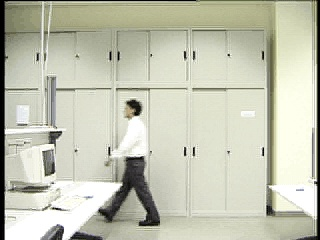
\includegraphics[width=1\linewidth]{figures/lab_0161.jpg}
  \caption{aton\_lab}
\end{subfigure}
\hfill
\begin{subfigure}{.49\linewidth}
  \includegraphics[width=1\linewidth]{figures/lab_gt_0161.jpg}
  \caption{aton\_lab ground truth}
\end{subfigure}
\hfill
\begin{subfigure}{.49\linewidth}
  \includegraphics[width=1\linewidth]{figures/lab_sat_bg_0161.jpg}
\end{subfigure}
\hfill
\begin{subfigure}{.49\linewidth}
  \includegraphics[width=1\linewidth]{figures/lab_sat_fg_0161.jpg}
\end{subfigure}
\hfill
\begin{subfigure}{.49\linewidth}
  \includegraphics[width=1\linewidth]{figures/lab_sat_bg_zoom_0161.jpg}
  \caption{Saturation channel (background)}
\end{subfigure}
\hfill
\begin{subfigure}{.49\linewidth}
  \includegraphics[width=1\linewidth]{figures/lab_sat_fg_zoom_0161.jpg}
  \caption{Saturation channel (frame)}
\end{subfigure}

\caption{The limited structural effects of cast shadows in the saturation channel (d).}
\label{fig:sat_struct}
\end{figure}

We attempt to characterize these localized changes in structure using HSV-SIFT, by detecting SIFT keypoints using only the saturation channels of both a frame and its corresponding background model. It is apparent that foreground objects introduce significant structural changes in any of the three channels, therefore the collection of SIFT descriptors is limited to only those considered \textit{low contrast}. The SIFT algorithm operates in four major stages: scale-space extrema extraction, elimination of low-contrast keypoints, elimination of strong edge responses, and the assignment of orientations. Low-contrast detections are eliminated due to their susceptibility to noise [ref SIFT]. In our study, we build two matrices: the first containing keypoints of low and normal contrast (still excluding edge responses), and the second containing only normal contrast keypoints. We then extract low-contrast keypoints using an exclusive-or operation. The non-linearity of light attenuation, paired with surface irregularities, make shadowed regions in the saturation channel ripe regions for low-contrast SIFT keypoints. When drawn onto the source frame, we can see that low-contrast SIFT keypoints align logically with shadowed regions (Figure \ref{fig:sat_lowc_kp}). 

\begin{figure}
  \centering
  \begin{subfigure}{.75\linewidth}
  \includegraphics[width=1\linewidth]{figures/lab_lowc_rgb_0161.jpg}
  \caption{Low-contrast SIFT keypoints detected using the intensity channel.}
\end{subfigure}
\hfill
\begin{subfigure}{.75\linewidth}
  \includegraphics[width=1\linewidth]{figures/lab_lowc_sat_0161.jpg}
  \caption{Low-contrast SIFT keypoints detected in the saturation channel.}
\end{subfigure}

\caption{Detecting low-contrast SIFT keypoints in the saturation channel more effectively captures structural changes due to cast shadows.}
\label{fig:sat_lowc_kp}
\end{figure}

With shadows partially characterized by low-contrast SIFT keypoints, this study utilizes this insight by attempting to model the proportion of foreground objects to shadows introduced in a given frame. The approximate ratio of shadows introduced to foreground objects in calculated for both the foreground and background frames, using the ratio:

\begin{equation}
\%lowC = 1 - \dfrac{num SIFT(0.04) features}{num SIFT(0.01) features}
\end{equation}

where \textit{SIFT(0.04)} represents features captured using the default contrast threshold (0.04), and \textit{SIFT(0.01)} represents features captured using a low contrast threshold. We then compare the \%\textit{lowC} ratios of the foreground to the background:

\begin{equation}
\%lowC(bg \rightarrow fg) = \dfrac{\%lowC(fg)}{\%lowC(bg)}
\end{equation}

This calculated ratio is used for improving and accentuating correlation of attenuation against algorithm parameters.

\section{Weak Detector Estimation - Creating a Model} \label{section:model}

\textbf{Wrote this first without knowing what the other sections would be. May require serious re-write}

With the coneR1 parameter tuned to optimal performance for a wide variety of datasets, we can begin to model a difference between environmental parameters and the optimal cone range. Normalizing correlative environmental parameters, we model an optimal shift from calculated parameters to the optimal value of the weak detector. While the average attenuation from the foreground to the background provides reasonable correlation to the weak detector's cone angle, said correlation does not indicate accurate magnitude for the environmentally-calculated cone angle parameter. This is due to the nature of the properties of attenuation. The attenuation calculation utilized is a function of brightness shift as a percentage of a background value, e.g., a pair of foreground/background pixels with a value of 50 and 100 produces the same attenuation as a pair valued at 50 and 25, respectively.

To circumvent this dilemma, required magnitude shift can be extrapolated from the magnitude of color shift found from foreground to background. From the color shift we can calculate brightness shift. By plotting the average brightness magnitude difference against the required shift of attenuation to optimal angle, we produce a general relationship between foreground attenuation, brightness magnitude, and the shift required to perform optimally. Using data points from each frame in each dataset, we can produce a best-fit polynomial to generalize a model of attenuation and brightness magnitude shift into a scene-generated cone angle parameter. To avoid over-fitting, a parametrized logarithm was chosen to represent the required magnitude shift ($\Delta$ RGB). Regression of our data is shown in Figure \ref{fig:polyfit}.

\begin{figure}
  \centering
  \includegraphics[width=1\linewidth]{figures/polyfit.jpg}
  \caption{Regression performed on RGB shift found per frame, vs. required magnitude shift to optimal.}
  \label{fig:polyfit}
\end{figure}

The final equation to represent the newly calculated algorithmic parameter can be assembled as:

\begin{equation}
(1 - \Delta RGB)*(1 - \%fr \rightarrow bg) + Mag. Shift
\end{equation}

\end{document}
